
\documentclass[
  english,        % define the document language (english, german)
  font=libertine,     % define main text font (helvet, times, palatino, libertine)
  onecolumn,      % use onecolumn or twocolumn layout
]{tumarticle}

\usepackage{acro}
% Define all acronyms in this file
\DeclareAcronym{CRS}{short = CRS, long = Commercial Resupply Services}
\DeclareAcronym{ISS}{short = ISS, long = International Space Station}
\DeclareAcronym{MECO}{short = MECO, long = main engine cutoff}
\DeclareAcronym{SECO}{short = SECO, long = second-stage engine cutoff}
\DeclareAcronym{LOX}{short = LOX, long = liquid oxygen}
\DeclareAcronym{RP1}{short = RP-1, long = rocket propellant-1}
\DeclareAcronym{CG}{short = CG, long = center of gravity}
\DeclareAcronym{IMU}{short = IMU, long = inertial measurement unit}
\DeclareAcronym{GNSS}{short = GNSS, long = global navigation satellite system}
\DeclareAcronym{LIDAR}{short = LiDAR, long = light detection and ranging}
\DeclareAcronym{RMS}{short = RMS, long = root mean square}
\DeclareAcronym{MEKF}{short = MEKF, long = multiplicative extended Kalman filter}
\DeclareAcronym{ECEF}{short = ECEF, long = Earth-centred Earth-fixed frame}
\DeclareAcronym{ECI}{short = ECI, long = Earth-centred inertial frame}
\DeclareAcronym{NIS}{short = NIS, long = normalized innovation squared}
\DeclareAcronym{PSD}{short = PSD, long = power spectral density}


% load additional packages
\usepackage{lipsum}
\usepackage{booktabs}
\usepackage{svg}


% article metadata
\title{Falcon9 Simulation}
\subtitle{Topics in Aerospace Engineering - Team 5}

\author{Park Kwanwoo}
\author{Lambin Emilien}
\author{Bieser Philipp}

\date{\today}



\begin{document}


\maketitle
\tableofcontents

% +++++ Main part
% Chapter order follows the binding outline in AGENTS.md (adopted from
% PROPOSED_OUTLINE.md). Commented lines mark chapters not yet written.
\section{Introduction and Project Scope}
\label{sec:introduction}

\subsection{Project 2 objectives}
Project 2 develops a physics-based Falcon 9 simulator and a navigation system driven by simulated sensor measurements. Forces, moments, changing mass properties, and numerical integration generate the vehicle motion; the navigation algorithm estimates states from imperfect observations of that motion. The course identifies this environment as the computational foundation for guidance design in Project 3 and integrated control in Project 4 \cite[slides 2--4]{project2}.

The assignment covers equations of motion and coordinate systems, gravity and atmosphere, propulsion and aerodynamics, mass/inertia variation, configuration changes, and estimation of position, velocity, attitude, and angular velocity. Its validation requirement combines representative flight phases, public flight-data comparisons, and navigation-error analysis \cite[slides 4--6]{project2}. Accordingly, the report distinguishes physical-model verification, agreement with external flight evidence, and estimation error relative to simulation truth. These comparisons establish different aspects of the simulator's credibility.

\subsection{CRS-10 selection and vehicle configuration}
CRS-10 is SpaceX's tenth contracted Dragon cargo-resupply mission to the International Space Station. The official mission material identifies a Falcon 9/Dragon launch from Launch Complex 39A, first-stage recovery at Landing Zone 1, and an approximate sequence of cutoff, separation, and restart events \cite{nasacrs10press}. The public technical webcast and its published ascent digitization provide an accessible reference for a quantitative comparison \cite{crs10webcast,crs10telemetry}.

The mission exercises three connected trajectory segments: common-stack ascent, first-stage return, and upper-stage continuation. It therefore tests configuration changes and inherited states as well as continuous motion. The Dragon payload also fixes the configuration choice: the model carries one loaded Dragon/trunk assembly rather than a generic satellite and fairing. NASA's $2490\,\mathrm{kg}$ cargo inventory is a subset of that loaded assembly, not its total mass \cite{nasacrs10overview}.

Figure~\ref{fig:crs10-context} identifies the selected hardware and official mission document. The press kit supplies mission context and approximate preflight timing; generic Falcon user guides supply supplementary geometry and operating-point evidence with their configuration/date limitations. Internal dimensions and mass properties require the evidence-qualified modeling described in the vehicle chapter.

\begin{figure}[!htbp]
\centering
\begin{minipage}[c]{0.57\linewidth}
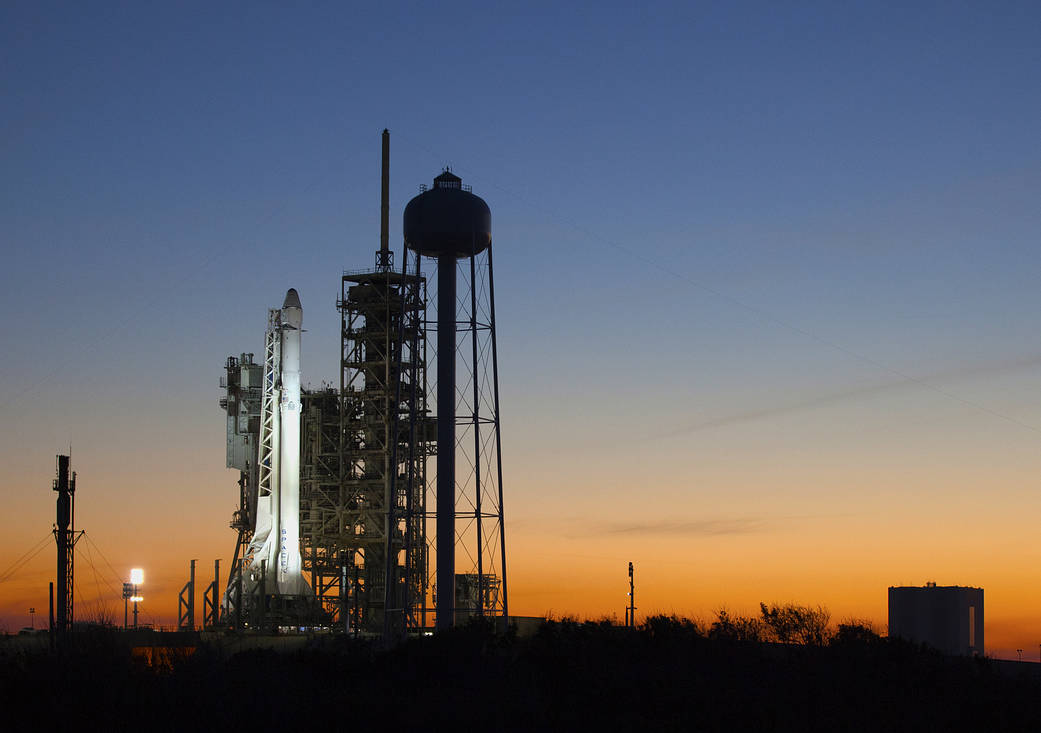
\includegraphics[width=\linewidth]{images/crs10_pad_nasa.jpg}
\end{minipage}\hfill
\begin{minipage}[c]{0.39\linewidth}
\centering
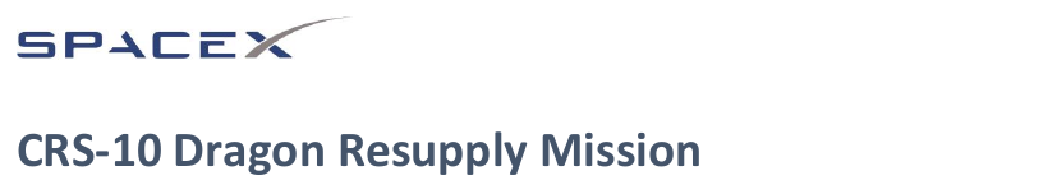
\includegraphics[width=\linewidth]{images/crs10_presskit_header.pdf}\\[1ex]
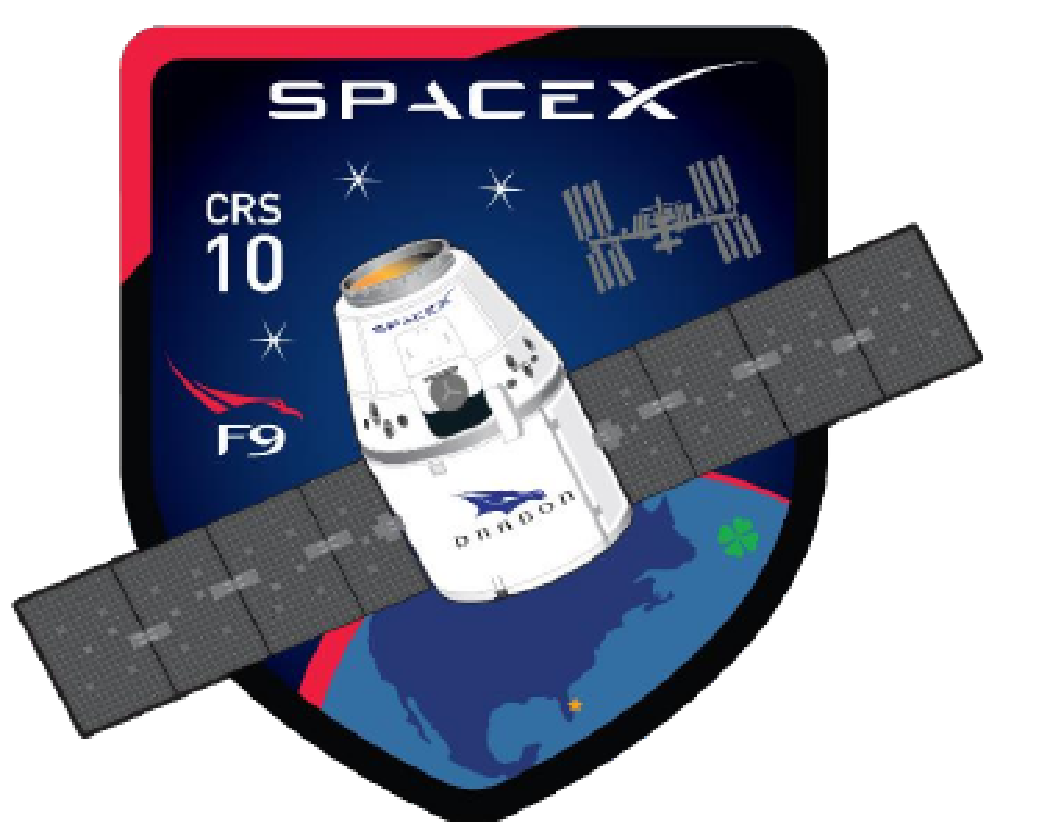
\includegraphics[width=0.60\linewidth]{images/crs10_mission_patch.pdf}
\end{minipage}
\caption{CRS-10 reference configuration. Left: Falcon 9 and Dragon at LC-39A before launch, NASA/Glenn Benson \cite{nasacrs10photo}. Right: header and mission-patch excerpts from the official SpaceX press kit \cite{nasacrs10press}. The images identify the hardware and source; they do not determine the internal mass distribution.}
\label{fig:crs10-context}
\end{figure}

\clearpage
\subsection{Simulation and validation scope}
The initial vehicle contains both stages and the loaded Dragon assembly. At separation, a conservative state map creates two children. The first stage proceeds through boostback, coast, entry burn, aerodynamic descent, landing burn, and first geometric contact. The upper child retains Dragon and continues under its own engine and attitude commands. Both children inherit the propagated separation state; a separately selected descent checkpoint does not create the full-return trajectory.

Flight commands provide a repeatable scenario for exercising the physical models. Scheduled reference times are distinguished from state-triggered return conditions, and project-designed return commands are classified as assumptions. The upper continuation demonstrates independent propagation rather than validated orbital insertion. First-stage navigation propagates its own quaternion from noisy gyros in a multiplicative extended Kalman filter (MEKF) with GNSS/LiDAR updates. A simulated star tracker supplies gated attitude observations; acceptance is checked per run. Physical attitude supplies sensor generation, an assumed initial alignment, and the evaluation reference; it is not continuously supplied to the active estimator.

External trajectory comparison uses the retained video-derived ascent observations over approximately $0$--$140\,\mathrm{s}$. Their classification is E: they are digitized public readouts, not released onboard telemetry. The ascent operating point and pitch timescale were adjusted using the same record, so their agreement is calibration evidence. Model-level tests, continuous state transfer, return/upper trajectories, and navigation errors provide additional evidence with their own stated assumptions. Navigation error against the simulator's truth does not by itself establish the accuracy of the physical vehicle model.
        % Ch 1
%\section{Simulation Architecture and Shared Conventions}
\label{sec:architecture}

\subsection{Physical truth, measurements, and estimates}
The physical branch computes loads and mass properties and integrates vehicle motion. The measurement branch samples that truth through sensor error and availability models. Navigation propagates its own attitude and estimates the IMU-station motion. Comparison uses the same station and time. Figure~\ref{fig:architecture} separates these interfaces.

\par\medskip\noindent\begin{minipage}{\linewidth}
\centering
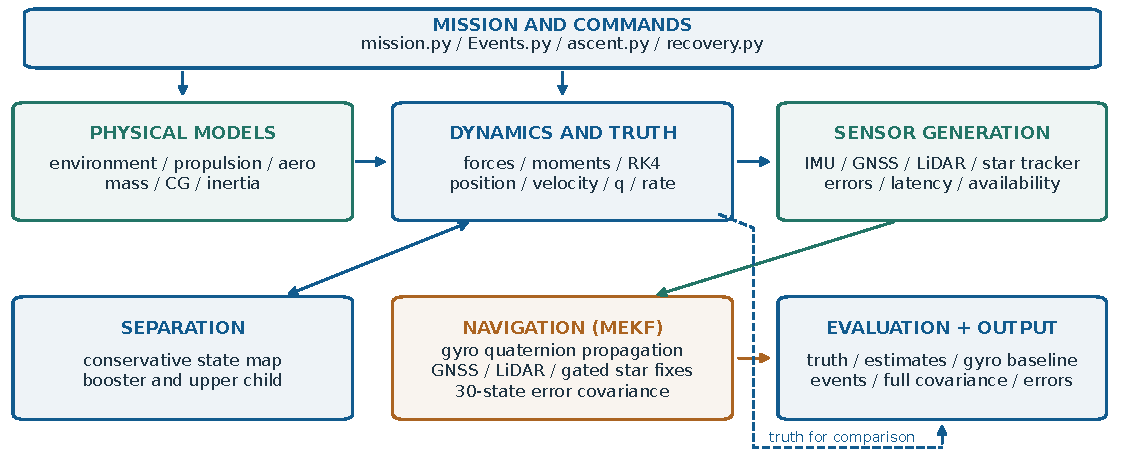
\includegraphics[width=0.97\linewidth]{images/simulation_architecture.pdf}
\captionof{figure}{Implemented data flow. The MEKF uses simulated sensor measurements and its own propagated attitude. Truth supplies sensor generation and evaluation; initial alignment is assumed. Return commands use physical-state feedback, while navigation is evaluated separately.}
\label{fig:architecture}
\end{minipage}\par\medskip

The mission layer selects the initial configuration, commands, and accepted phase. A throttle command becomes thrust and flow through propulsion; an aerodynamic configuration and fin command become force and moment through aerodynamics. The dynamics model then calculates the resulting motion. Neither the force provider nor the mass model prescribes the reference altitude/speed history. Table~\ref{tab:architecture-modules} assigns the corresponding implementation responsibilities.

\par\medskip\noindent\begin{minipage}{\linewidth}
\centering\small
\begin{tabularx}{\linewidth}{@{}p{0.22\linewidth}p{0.35\linewidth}X@{}}
\toprule
Function & Main modules & Interface \\
\midrule
Vehicle properties & \path{VehicleData.py}\newline\path{vehicle_mass_model.py}\newline\path{mass_properties.py} & Trial inventory to mass, CG, inertia, and derivatives. \\
Environment and loads & \path{Environement.py}\newline\path{propulsion.py}\newline\path{Aerodynamics.py}\newline\path{load_interface.py} & Trial state/commands to loads and exhaust data. \\
Motion and configuration & \path{dynamics.py}\newline\path{frames.py}\newline\path{staging.py} & Derivative, integrated state, and inherited child states. \\
Measurement and estimation & \path{sensors.py}\newline\path{kalman.py} & Sensor-station truth to observations and separate estimates. \\
Mission execution & \path{main.py}\newline\path{mission.py}\newline\path{Events.py} & Commands, accepted clocks/events, state synchronization, and saved output. \\
\bottomrule
\end{tabularx}
\captionof{table}{Responsibilities of the shared implementation. Configuration and scenario decisions are kept separate from reusable component arithmetic and equations of motion.}
\label{tab:architecture-modules}
\end{minipage}\par\medskip

\subsection{Frames, origins, and attitude convention}
Frame $B$ is right-handed and fixed to the vehicle, with $+x_B$ toward the nose. Frame $E$ is Earth-centred, launch-aligned, and rotating with Earth. Code identifiers call it ECEF, but its axes are not conventional Greenwich-axis ECEF. At the launch site, $+x_E$ is north, $-y_E$ east, and $+z_E$ up; the initial structural base is $[0,0,R_E]^{\mathsf T}$ with $R_E=6371000\,\mathrm{m}$.

The scalar-first Hamilton quaternion $\vect q_{BE}=[q_w,q_x,q_y,q_z]^{\mathsf T}$ maps Body components into $E$ using $\mat C_{BE}$. Equation~\eqref{eq:frame-initialization} defines the vector transformation and launch orientation:
\begin{equation}
 \vect u^E=\mat C_{BE}\vect u^B,\qquad
 \vect q_{BE}(0)=\begin{bmatrix}\sqrt{1/2}&0&-\sqrt{1/2}&0\end{bmatrix}^{\mathsf T},
 \qquad
 \mat C_{BE}(0)=\begin{bmatrix}0&0&-1\\0&1&0\\1&0&0\end{bmatrix}.
\label{eq:frame-initialization}
\end{equation}
Thus Body $+x$ is initially upward, Body $+y$ maps to $+y_E$, and Body $+z$ maps to $-x_E$. Quaternions are normalized, and $\vect q$ and $-\vect q$ denote the same orientation. The adopted latitude $\lambda=28.6^\circ$ rotates the Earth-rate vector into the launch-aligned frame as $\vect\Omega^E=\Omega_E[\cos\lambda,0,\sin\lambda]^{\mathsf T}$, with $\Omega_E=7.292115\times10^{-5}\,\mathrm{rad\,s^{-1}}$. It does not relocate the pad into Greenwich-axis coordinates.

Reference point and component basis are separate choices. Table~\ref{tab:state-origins} distinguishes them. A structural station $\vect s^B$ is measured from the stage base, whereas the corresponding CG force arm is $\vect d^B=\vect s^B-\vect c^B$, where $\vect c^B$ is the current CG station.

\begin{table}[!htbp]
\centering\small
\begin{tabularx}{\linewidth}{@{}p{0.31\linewidth}X@{}}
\toprule
Quantity & Meaning \\
\midrule
Dynamic position $\vect r_C^B$ & Earth centre to instantaneous CG, expressed in current Body axes. \\
Dynamic velocity $\vect v_C^B$ & CG velocity relative to rotating Earth, in current Body components. \\
Vehicle-object position/velocity & Structural-base state, with the same external origin and Body component basis. \\
Component/sensor station $\vect s^B$ & Fixed structural location measured from the relevant stage base. \\
Moment and inertia & About the instantaneous vehicle CG, in Body axes. \\
Filter position/velocity & At the fixed IMU station, expressed in frame $E$. \\
\bottomrule
\end{tabularx}
\caption{Shared origins and representations. Storing an Earth-centred vector in Body components does not make its origin the CG.}
\label{tab:state-origins}
\end{table}

\subsection{Physical and estimated states}
The physical state contains 15 stored numbers: three CG-position components, three CG-velocity components, four quaternion components, three angular-rate components, and two stage-indexed propellant inventories. The unit-quaternion constraint leaves three independent attitude coordinates. Each separated child retains the same state layout, with the detached stage's inventory set to zero.

The active MEKF maintains nominal IMU-station position and velocity in $E$, Body-frame accelerometer bias, the unit quaternion, gyro bias, three gyro scale factors, and six off-diagonal gyro calibration terms. Its covariance represents a 24-component error state: position, velocity, accelerometer bias, small-angle attitude error, gyro bias, scale factors, and misalignment terms. The quaternion occupies four nominal numbers but only three attitude-error coordinates. The original nine-state, supplied-attitude mode remains an optional diagnostic; it is not the default run.

Noisy gyro samples propagate the estimated quaternion using the same Body-to-$E$ convention as Equation~\eqref{eq:frame-initialization}. GNSS and LiDAR update the coupled estimate; the star-tracker correction is conditional on availability and an innovation gate. Measured rate, estimated gyro bias, and the calibration matrix form the angular-rate estimate; rate is not a separate dynamic filter state. An independent, unaided gyro quaternion provides a drift baseline. The default initial attitude equals the launch alignment, an A-class initialization assumption. The filter does not receive physical attitude during propagation or correction. Calibration-state estimation does not by itself demonstrate identifiability; the nominal run injects gyro bias and noise but zero scale-factor and misalignment errors.

The assumed first-stage stations are $[38,0,0]^{\mathsf T}\,\mathrm{m}$ for the IMU, $[41,0,0]^{\mathsf T}\,\mathrm{m}$ for GNSS, and $[0.5,0,0]^{\mathsf T}\,\mathrm{m}$ for LiDAR. These are A-class experiment settings. They remain on the structure when the CG moves or the upper stage separates. The ideal sensor state follows the structural-point kinematics; sensor errors are added afterward. An estimate at the IMU station is therefore compared with truth at that station, not with the changing geometric CG.

The stored angular rate and simulated ideal gyro use the Body-relative-to-$E$ rate. A physical inertial gyro instead senses Body-relative-to-inertial rotation; the present sensor convention omits that Earth-rate difference. The star-tracker interface explicitly rotates between $E$ and an inertial frame that coincides with $E$ at launch. This conversion does not change the gyro convention. Translation includes Coriolis and centrifugal acceleration; a fully physical inertial strapdown model requires a corresponding gyro Earth-rate treatment.

The star tracker is an A-class simulated aiding sensor, not evidence of CRS-10 flight hardware. Its defaults are $4\,\mathrm{Hz}$, $0.1\,\mathrm{s}$ latency, $5$ arcsec cross-boresight and $40$ arcsec boresight-roll standard deviations, a $60\,\mathrm{km}$ minimum altitude, and a $2\,\mathrm{deg\,s^{-1}}$ rate limit. The reviewed seed-1 full-flight run rejects all available star-tracker fixes at the innovation gate. Its measured performance therefore characterizes gyro/GNSS/LiDAR estimation. Sensor and filter chapters must distinguish an implemented correction interface from accepted aiding and assess covariance consistency alongside point-estimate errors.

\subsection{Load and execution interfaces}
The load record separates nongravitational force in newtons, CG moment in newton-metres, central gravity in $\mathrm{m\,s^{-2}}$, rotating-frame acceleration in $\mathrm{m\,s^{-2}}$, nonnegative stage consumption in $\mathrm{kg\,s^{-1}}$, and nozzle-exit flow data. Station forces contribute $\vect d\times\vect F$ once; free aerodynamic/control moments are supplied separately. Gravity and frame acceleration are added once in the dynamics, rather than included again in the force sum.

At each RK4 trial evaluation, properties and loads are recomputed from the trial state without advancing accepted vehicle inventories, event order, or sensor random generators. The mission loop synchronizes accepted states and samples due sensors. Steps are shortened at relevant command, event, sensor, and output boundaries. At separation, the same first-stage sensor/filter objects continue while two physical children inherit the parent state. The upper child is propagated independently on the common mission clock. Detailed command laws and scheduling belong to mission execution; these interfaces define what the models exchange.
       % Ch 2 - to be written
\section{Vehicle, Stages and Mission}
\label{sec:vehicle}

The simulator follows the Falcon 9 launch vehicle in the configuration flown
on SpaceX CRS-10, the tenth Commercial Resupply Services mission to the
International Space Station (launched 19 February 2017 from Launch
Complex~39A; the first stage returned to a landing site near the pad)
\cite{nasacrs10press}. The model is not a reconstruction of flight
hardware: it is a project-configured representation assembled from
published sources. Every adopted parameter value therefore carries an
evidence class --- K (authoritative known value), E (literature estimate)
or A (explicit modeling assumption) --- and the tables in this report state
the class of every value. The underlying records are
\texttt{data/vehicle\_parameters.json} (parameter set and sources) and
\texttt{data/crs10\_mission.json} (mission configuration).

\subsection{Vehicle configuration and stages}

The modeled vehicle is a two-stage stack of $62.4\,\mathrm{m}$ model height:
stage~1 ($42.6\,\mathrm{m}$), stage~2 ($12.6\,\mathrm{m}$), and the
Dragon~spacecraft with its trunk represented as one uniform assembly of
$7.2\,\mathrm{m}$ equivalent length and $1.83\,\mathrm{m}$ equivalent
radius. All axial stations are measured from the structural base of the
referenced stage along the vehicle's Body $+x$ axis (toward the nose).
Table~\ref{tab:vehicle} lists the adopted geometry and mass values.

\begin{table}[htbp]
\centering
\begin{tabular}{lrl}
\toprule
Component & Value & Class \\
\midrule
Outer diameter & $3.66\,\mathrm{m}$ & K \\
Stage-1 length & $42.6\,\mathrm{m}$ & E/A \\
Stage-2 length & $12.6\,\mathrm{m}$ & E/A \\
Dragon$+$trunk equivalent length & $7.2\,\mathrm{m}$ & E/A \\
Model total height & $62.4\,\mathrm{m}$ & E/A \\
Stage-1 dry mass & $22\,200\,\mathrm{kg}$ & E \\
Stage-1 propellant load & $410\,900\,\mathrm{kg}$ & E \\
Stage-2 dry mass & $4\,000\,\mathrm{kg}$ & E \\
Stage-2 propellant load & $107\,500\,\mathrm{kg}$ & E \\
Dragon loaded assembly (incl.\ cargo) & $8\,430\,\mathrm{kg}$ & E \\
Launch mass (model sum) & $553\,030\,\mathrm{kg}$ & E/A \\
Stage-1 dry CG station above base & $17.52\,\mathrm{m}$ & E/A \\
Stage-1 dry inertia $[I_{xx},I_{yy},I_{zz}]$ & $[61\,368.59, 4\,441\,994.04, 4\,441\,994.04]$\,$\mathrm{kg\,m^2}$ & E/A \\
\bottomrule
\end{tabular}
\caption{Vehicle geometry and mass model with evidence classes. Stage
lengths combine legacy Full Thrust geometry with a contiguous-stage model;
the Dragon assembly mass (including $2\,490\,\mathrm{kg}$ of cargo
\cite{nasacrs10overview}) is an external estimate
\cite{kyledatasheet}. Sources: geometry and dry/propellant masses
\cite{spacexguide2025,pezent2024,crs1presskit}.}
\label{tab:vehicle}
\end{table}

Inside stage~1, the RP-1 tank occupies the axial interval
$x = 4.0$--$18.7\,\mathrm{m}$ and the LOX tank $x = 18.7$--$40.8\,\mathrm{m}$;
the liquids are modeled as settled flat cylinders at constant densities
($820\,\mathrm{kg/m^3}$ for RP-1, $1\,250\,\mathrm{kg/m^3}$ for LOX). The
stage-1 dry mass contains a residual hardware budget of $6\,450\,\mathrm{kg}$
distributed uniformly over $x = 4.0$--$40.8\,\mathrm{m}$, since no surveyed
location exists; if that budget were free to move within its interval, the
dry CG station would shift between $12.18\,\mathrm{m}$ and $22.87\,\mathrm{m}$.
This range is a conditional spread of the placement assumption, not a
confidence interval. Tank geometry, depletion and the resulting CG and
inertia migration are treated in the propulsion and mass model chapter of
this report.

\subsection{Propulsion inventory}

Stage~1 carries nine Merlin 1D SL engines on a $1.3\,\mathrm{m}$ radius
ring (A); stage~2 carries a single MVac engine. Engine thrust application
(pivot) stations are $1.0\,\mathrm{m}$ and $0.5\,\mathrm{m}$ above the
respective stage base (A), and the gimbal limit is
$5^{\circ}$ (A). The model derives the vacuum thrust from the historical
sea-level operating point of $756\,\mathrm{kN}$ per engine
\cite{spacex2015} using the nozzle exit area $A_e$ and sea-level pressure
$p_0 = 101\,325\,\mathrm{Pa}$:
%
\begin{equation}
\label{eq:thrust-vac}
T_{\mathrm{vac}} = T_{\mathrm{sl}} + A_e \, p_0,
\qquad
I_{\mathrm{sp,sl}} = I_{\mathrm{sp,vac}} \, \frac{T_{\mathrm{sl}}}{T_{\mathrm{vac}}}
\end{equation}
%
which yields $824.901\,\mathrm{kN}$ and $285.023\,\mathrm{s}$
(respectively $935\,\mathrm{kN}$ and $348\,\mathrm{s}$ for the
literature-sourced MVac). Table~\ref{tab:engines} summarizes the engine set;
none of these values is a certified CRS-10 engine rating.

\begin{table}[htbp]
\centering
\begin{tabular}{lcc}
\toprule
Parameter & Merlin 1D SL ($\times 9$) & MVac ($\times 1$) \\
\midrule
Sea-level effective thrust & $756.000\,\mathrm{kN}$ (E/A) & --- \\
Vacuum thrust & $824.901\,\mathrm{kN}$ (E/A) & $935\,\mathrm{kN}$ (E) \\
Vacuum specific impulse & $311\,\mathrm{s}$ (E) & $348\,\mathrm{s}$ (E) \\
Sea-level specific impulse & $285.023\,\mathrm{s}$ (E/A) & --- \\
Nozzle exit area & $0.68\,\mathrm{m^2}$ (E) & $4.90\,\mathrm{m^2}$ (E) \\
Minimum throttle & $60\,\%$ (E) & $40\,\%$ (E) \\
\bottomrule
\end{tabular}
\caption{Engine model with evidence classes. The sea-level operating point
is a historical SpaceX value \cite{spacex2015}; engine data and throttle
limits are research-model estimates \cite{pezent2024}, not certified flight
limits.}
\label{tab:engines}
\end{table}

The initial stage-1 inventory is $123\,500\,\mathrm{kg}$ of RP-1 and
$287\,400\,\mathrm{kg}$ of LOX \cite{romerocalco2023} (loaded O/F mass
ratio $2.327$), while the consumption model uses a constant O/F mass ratio
of $2.35$ \cite{bykerk2023}. The adopted pair depletes LOX before RP-1 and
leaves $1\,202.13\,\mathrm{kg}$ of RP-1 at the mathematical burn limit.
This residual is a consequence of the adopted inventory/ratio combination,
not a known Falcon~9 landing reserve; independent tank states would be
required for variable O/F, venting or refilling.

\subsection{Return propellant budget}

The first-stage return reserves propellant by planning allocation (all
class A): $38\,\mathrm{t}$ for the boostback burn, $16\,\mathrm{t}$ for the
entry burn, $10\,\mathrm{t}$ for the landing burn, and a protected reserve of
$2\,\mathrm{t}$. Unused boostback and entry allocations transfer to the
landing burn; the reserve and the limiting-tank residual are never
consumed. These are planning budgets, not measured characteristics of the
CRS-10 vehicle.

\subsection{Mission phases and flight paths}

The mission executes as an event-driven phase sequence: each transition
carries a condition (a fixed reference time, or a guard signal such as
altitude, speed, propellant state or landing prediction) and is checked
against the accepted integration state. The ascent commands
MECO at $140\,\mathrm{s}$ (with a $1\,\mathrm{s}$ shutdown ramp) and
separation at $144\,\mathrm{s}$; these are approximate published preflight
times adopted as commands \cite{nasacrs10press}. All later event times are
simulated outcomes of the model, not observed CRS-10 event times.
Table~\ref{tab:phases} lists the nominal phases of the full mission.

\begin{table}[htbp]
\centering
\begin{tabular}{lll}
\toprule
Phase & Transition condition & Nominal time\, [s] \\
\midrule
Powered ascent & Liftoff initial state & $0$ \\
Shutdown ramp / MECO & Fixed command, $1\,\mathrm{s}$ ramp & $140.00$--$141.00$ \\
Full-stack coast & Zero thrust and propellant flow & $141.00$--$144.00$ \\
Stage separation & Zero flow, engines off & $144.00$ \\
Boostback burn & Ignition after fuel and attitude checks & $161.00$--$208.81$ \\
Return coast & --- & $208.81$--$370.14$ \\
Entry burn & Descending through $45\,\mathrm{km}$; ends at $500\,\mathrm{m/s}$ & $370.14$--$392.95$ \\
Aerodynamic descent & --- & $392.95$--$426.16$ \\
Landing burn & Predicted stopping clearance $+\,1.5\,\mathrm{km}$ & $426.16$--$465.08$ \\
Touchdown & Lowest leg tip reaches the ground sphere & $465.083$ \\
\bottomrule
\end{tabular}
\caption{Mission phases of the full simulation case. Times after boostback
ignition are simulated outcomes (nominal run, seed 1); the ascent times are
adopted reference commands.}
\label{tab:phases}
\end{table}

Three flight paths leave the pad together and diverge at separation
(Figure~\ref{fig:flightpaths}). The full stack ascends to MECO and
separates; the separated upper stage (stage 2 with the Dragon assembly)
ignites $8\,\mathrm{s}$ after separation and, under its assumed command
sequence, shuts down at SECO $545\,\mathrm{s}$ at about
$200\,\mathrm{km}$ altitude and $1\,600\,\mathrm{km}$ surface distance
from the launch site. The booster flies the return arc: after boostback it
coasts to an apogee of about $111.5\,\mathrm{km}$ at roughly
$90\,\mathrm{km}$ surface distance, descends through the entry burn and the
aerodynamic descent, and lands at the assumed ground target
$14.0\,\mathrm{km}$ south and $6.0\,\mathrm{km}$ east of the launch site
(the nominal run reaches that target within meters). The upper-stage
commands are demonstration assumptions (A), not reconstructed flight data;
quantitative comparison of the ascent against the video-derived telemetry
record and the landing acceptance metrics are discussed in the results
chapter of this report.

\begin{figure}[htbp]
\centering
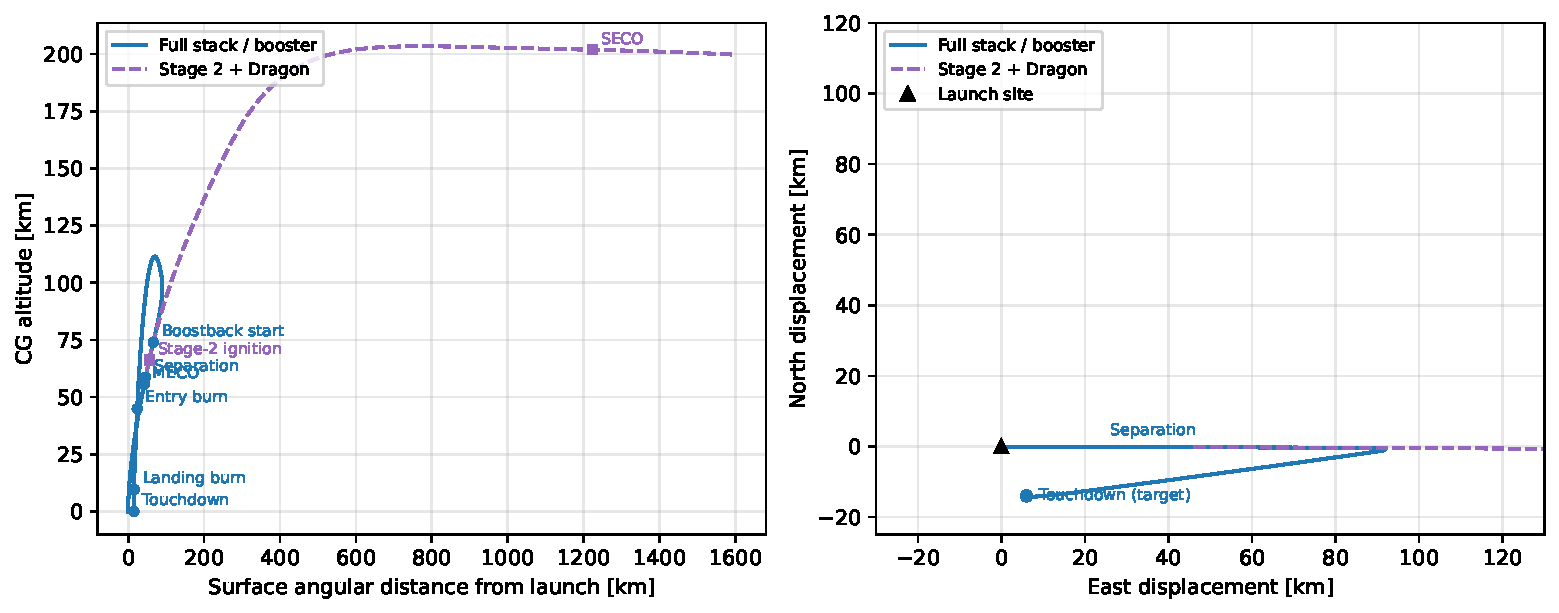
\includegraphics[width=\linewidth]{images/flight_paths.pdf}
\caption{Simulated flight paths of the nominal full-mission run (seed~1).
Left: CG altitude against surface angular distance from the launch site.
Right: ground displacement; the launch site is at the origin and the
assumed landing target lies $14.0\,\mathrm{km}$ south and
$6.0\,\mathrm{km}$ east of it. Markers denote mission events.}
\label{fig:flightpaths}
\end{figure}
     % Ch 3 seed - to be merged into content/vehicle_dynamics.tex
\section{Environment Models}
\label{sec:environment}

The environment module (\texttt{Environement.py}) is a pure service layer:
it supplies the world the vehicle flies through and never calls back into
vehicle, dynamics or control code. Its services are the standard atmosphere,
point-mass gravity with its gradient, the acceleration of the rotating
Earth-fixed frame, the wind, and the ground reference; all evaluations are
stateless functions of the current state. Following the project convention,
any state outside a modeled domain is rejected with an error, never
extrapolated.

\subsection{Atmosphere}

The atmosphere follows the US Standard Atmosphere 1976 \cite{ussa1976}:
seven gradient layers between sea level and the mesopause at
$84.852\,\mathrm{km}$, reproduced layer by layer. Within a layer with base
temperature $T_b$, base pressure $p_b$ and lapse rate $L$, and in the
isothermal case, the pressure is
%
\begin{equation}
\label{eq:atmosphere-pressure}
p(h) = p_b \left( \frac{T_b + L\,(h - h_b)}{T_b} \right)^{-\frac{g_0}{R\,L}}
\quad (L \neq 0),
\qquad
p(h) = p_b \, \exp \left( -\frac{g_0\,(h - h_b)}{R\,T_b} \right)
\quad (L = 0),
\end{equation}
%
with $g_0 = 9.80665\,\mathrm{m/s^2}$ and the gas constant of dry air
$R = 287.05287\,\mathrm{J/(kg\,K)}$. Density and speed of sound follow the
ideal-gas and isentropic relations,
$\rho = p/(R\,T)$ and $a = \sqrt{\gamma R T}$ with $\gamma = 1.4$.
Sea-level values are $T = 288.15\,\mathrm{K}$,
$p = 101\,325\,\mathrm{Pa}$, $\rho = 1.225\,\mathrm{kg/m^3}$.

Above the mesopause the model deliberately stops claiming physics: an
isothermal tail at $T_m = 186.946\,\mathrm{K}$ decays exponentially with a
scale height of $R\,T_m/g_0 \approx 5.47\,\mathrm{km}$ toward numerical
vacuum (density below $10^{-150}\,\mathrm{kg/m^3}$ at the
$2\,000\,\mathrm{km}$ envelope ceiling; $p(200\,\mathrm{km}) \approx
2.7\times10^{-10}\,\mathrm{Pa}$). The envelope
$0$--$2\,000\,\mathrm{km}$ is the mission scope; altitudes outside raise a
domain error instead of a number. Figure~\ref{fig:environment-models}
shows the model against the published USSA 1976 checkpoint values that the
test suite pins ($5$--$80\,\mathrm{km}$, altitudes, temperatures,
pressures and densities compared at $5\times10^{-5}$ relative tolerance).
The environment suite of $41$ tests additionally checks layer-boundary
continuity, monotone pressure and density decay, exact tail scale height,
and hydrostatic balance $\partial p/\partial h = -g_0\,\rho$ inside every
layer.

\begin{figure}[htbp]
\centering
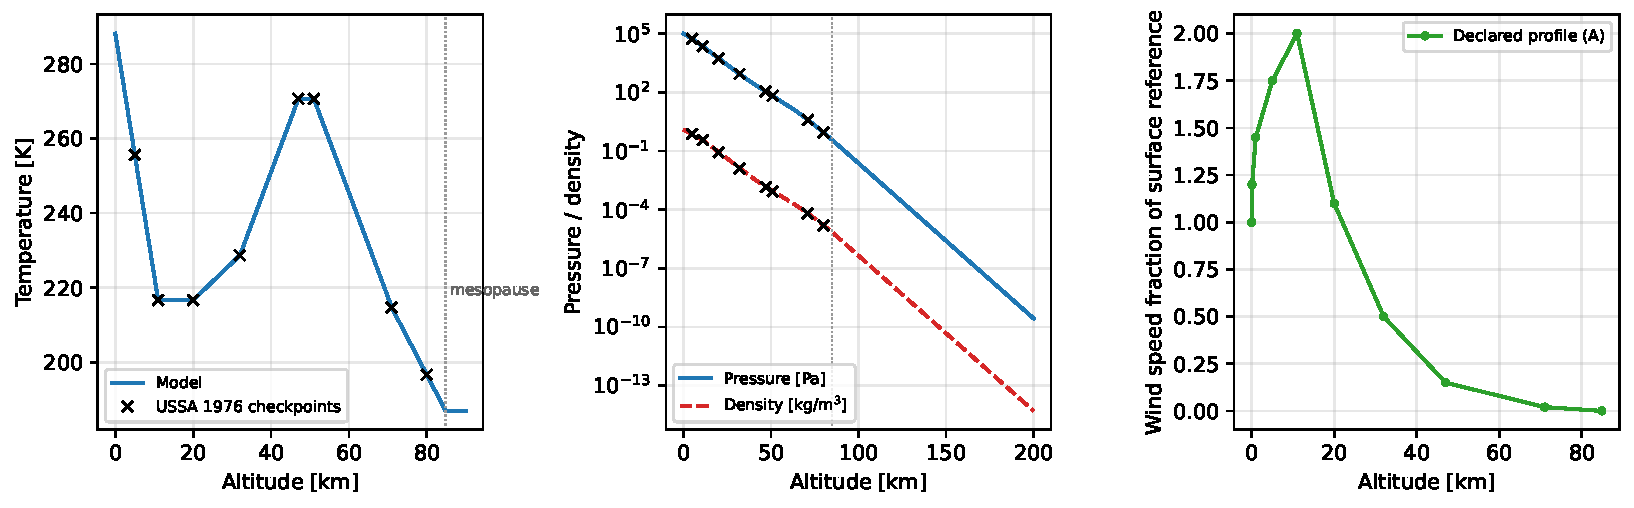
\includegraphics[width=\linewidth]{images/environment_models.pdf}
\caption{Environment model. Left: layer temperatures to the mesopause
with published USSA 1976 checkpoint values. Center: pressure and density
(logarithmic) to $200\,\mathrm{km}$, showing the isothermal tail above
the mesopause; black markers are the published checkpoints. Right: the
declared wind-profile scale factor of the surface reference wind (class
A), which is zero above the modeled atmosphere; the nominal mission runs
in calm air.}
\label{fig:environment-models}
\end{figure}

\subsection{Gravity and rotating-frame accelerations}

Gravity is the reduced Newtonian point-mass model. With the Earth radius
$R_E = 6\,371\,\mathrm{km}$ and the configured surface gravity $g_0$, the
gravitational parameter is $\mu = g_0 R_E^2$, so the gravitational
acceleration at the launch site is the configured value by construction:
%
\begin{equation}
\label{eq:gravity}
\mathbf{a}_g = -\,\frac{\mu}{\|\mathbf{r}\|^3}\,\mathbf{r}.
\end{equation}
%
Gravity never appears as a force; Equation~\eqref{eq:gravity} is added
once as an acceleration next to thrust over mass. The module also provides
the $3\times3$ gravity-gradient map
$\nabla_{\mathbf{r}}\mathbf{a}_g = (\mu/\|\mathbf{r}\|^3)\,
(3\,\hat{\mathbf{r}}\hat{\mathbf{r}}^{\mathsf{T}} - \mathbf{I})$, used only
in the navigation filter's prediction Jacobian (the navigation chapter),
not for torques. Oblateness ($J_2$) is out of scope.

The external frame is Earth-centred and launch-aligned (detailed in the
reference-frames chapter of this report); it does not rotate for the
flight mechanics themselves. Earth rotation enters translation only,
through the separate frame acceleration
%
\begin{equation}
\label{eq:frame-acceleration}
\mathbf{a}_{\mathrm{fr}} = -2\,\boldsymbol{\omega}_E \times \mathbf{v}
\;-\; \boldsymbol{\omega}_E \times
(\boldsymbol{\omega}_E \times \mathbf{r}),
\end{equation}
%
the Coriolis and centrifugal terms for velocity relative to the rotating
Earth, with the rotation vector
$\boldsymbol{\omega}_E = \Omega\,(\cos\varphi,\, 0,\, \sin\varphi)$ at
launch latitude $\varphi$. The nominal mission uses the sidereal rate
$\Omega = 7.2921150\times10^{-5}\,\mathrm{rad/s}$ at
$\varphi = 28.6^{\circ}$; setting $\Omega = 0$ disables the terms. The
frame accelerations, and their analytical gradients, are supplied once
per integration step next to gravity. The angular equations and the gyro
model retain the project's approximate Earth-rate treatment: no complete
inertial-rate coupling is claimed.

\subsection{Wind and ground reference}

The wind model is a surface reference vector (ECEF components in the
mission configuration) that can be rotated about the launch-site vertical,
scaled by a declared altitude profile: the scale factor of the surface
reference grows through the boundary layer, peaks at $2.0$ around the
$11\,\mathrm{km}$ jet-stream core, decays through the stratosphere and
reaches exactly zero at the mesopause --- there is no wind above the
modeled atmosphere (Figure~\ref{fig:environment-models}, right). The
profile is a declared stylization (class A). There are no gusts, no time
dependence and no direction shear, and the wind enters the physics only
through the relative-velocity term of the aerodynamics model. The nominal
full-mission run uses calm air: the mission configuration sets no surface
reference wind, so the default zero vector applies throughout.

The ground is a bare sphere of radius $R_E$; altitude is measured radially
above it, with an optional reference-level shift, and supports a station
offset from the center of gravity (used, for example, for engine-exit
altitude). Terrain and contact forces are out of scope; contact is
evaluated at the mission level through the leg-tip geometry discussed with
the landing criteria in the return-control chapter of this report.

The module validates its configuration at construction: non-finite
gravity, radius, ground offset or wind, non-positive radius, a negative
rotation rate or a latitude beyond $\pm 90^{\circ}$ all raise an error
before flight, not mid-integration.
  % Ch 4
\section{Aerodynamics}
\label{sec:aero}

\path{Aerodynamics.py} returns Body-frame forces and CG moments using the evidence-qualified register \path{data/aero_configurations.json}. Four configurations serve stack/booster phases; a fifth, \texttt{second\_stack}, is declared but not selected by the independent upper-stage drag provider (Section~\ref{sec:mission-exec}).

\subsection{Flow state and force build-up}

Equation~\eqref{eq:aero-flow} defines the relative flow and total angle:
%
\begin{equation}
\label{eq:aero-flow}
\mathbf{v}_{\mathrm{rel}} = \mathbf{v}_{\mathrm{CG}}
- \dot{\mathbf{c}} - \mathbf{w},
\qquad
\alpha = \operatorname{atan2}\bigl(\, \lVert \mathbf{v}_{\mathrm{rel},yz}\rVert, \; v_{\mathrm{rel},x} \,\bigr),
\end{equation}
%
where $\dot{\mathbf{c}}$ is the axial center-of-gravity migration rate
(Section~\ref{sec:vehicle}, stage depletion) and $\mathbf{w}$ the wind in
Body components (Section~\ref{sec:environment}). The total flow angle
$\alpha$ spans $0$ (nose-first) to $\pi$ (engine-first); every direction in
the lateral plane is handled, not only a pitch plane. The dynamic pressure
is $\bar{q} = \tfrac{1}{2}\,\rho\,v_{\mathrm{rel}}^2$ with the atmosphere
state of Section~\ref{sec:environment}.

The axial and potential-normal loads follow Equation~\eqref{eq:aero-axial-normal}; side segments add the crossflow terms of Equation~\eqref{eq:aero-crossflow}:
%
\begin{equation}
\label{eq:aero-axial-normal}
F_x = -\,\bar{q}\, S_{\mathrm{ref}}\, CA_0(M)\,\cos\alpha
\,|\!\cos\alpha|,
\qquad
N = \bar{q}\, S_{\mathrm{ref}}\, C_{N\alpha}\, \sin\alpha
\,|\!\cos\alpha|,
\end{equation}
%
\begin{equation}
\label{eq:aero-crossflow}
D_i = \bar{q}\; C_{Dc,i}\, S_i \,\sin^2\alpha
\qquad \text{per side segment } i,
\end{equation}
%
Reference areas/lengths appear in Table~\ref{tab:aero-configurations}. Normal force opposes lateral flow at a windward-end station (57.6 m for the stack, 41.0 m for the booster), mirrored about CG for retro flow. Crossflow forces act at side-area centroids. The landing configuration adds fin and deployed-leg segments to the body model.

The $\cos\alpha|\cos\alpha|$ factor reverses the axial load and fixed-deflection fin effect in engine-first flight and makes them vanish at $90^\circ$. Station moments are assembled once as $(\vect s-\vect c)\times\vect F$. Geometry determines restoring or destabilizing effects; the model does not impose passive stability.

Equation~\eqref{eq:aero-damping} closes the moment set with per-axis damping:
%
\begin{equation}
\label{eq:aero-damping}
\mathbf{M}_{\mathrm{damp}} = \operatorname{diag}(c_l,c_m,c_m)\,
\frac{\bar{q}\, S_{\mathrm{ref}}\, L_{\mathrm{ref}}^2}{2\,v_{\mathrm{rel}}}
\;\boldsymbol{\omega},
\end{equation}
%
with pitch and yaw coefficient $c_m$ tied by symmetry and roll coefficient $c_l$ separate (declared values: $-10$ full stack, $-20$ booster, roll $-3$ with fins
deployed; a zero coefficient means that no roll-damping contribution is applied).

\subsection{Configurations and axial curves}

\par\medskip\noindent\begin{minipage}{\linewidth}
\centering
\begin{tabular}{llrrl}
\toprule
Configuration & Phase & $S_{\mathrm{ref}}$ [m$^2$] & $L_{\mathrm{ref}}$ [m] & Axial curve / fins \\
\midrule
\texttt{full\_stack} & launch to separation & 21.08 & 62.4 & sourced $M\,0$--$7$; declared $M\,7$--$10$ \\
\texttt{booster\_alone} & coast, boostback & 10.52 & 42.6 & declared ($\pm 50\,\%$) \\
\texttt{booster\_return} & entry burn, descent & 10.52 & 42.6 & declared; four fins \\
\texttt{booster\_landing} & landing burn & 10.52 & 42.6 & declared; four fins and legs \\
\texttt{second\_stack} & stage-2 body (declared) & 10.52 & 19.8 & declared, sleeker estimate \\
\bottomrule
\end{tabular}
\captionof{table}{The five aerodynamic configurations. Station datum is the
configuration's own structural base. Fins deploy after boostback; the legs
deploy at landing ignition, which is represented by the segment difference
between \texttt{booster\_return} and \texttt{booster\_landing}.}
\label{tab:aero-configurations}
\end{minipage}\par\medskip

Figure~\ref{fig:aero-axial-curves} shows the adopted $CA_0(M)$ curves. The full-stack curve to Mach 7 is read from Pezent's RasAeroII analysis of a Falcon-9-like stack with fairing \cite{pezent2024}; its transonic peak is about 1.16 near Mach 1.06. The extension to Mach 10 and all booster/upper curves are engineering estimates, with declared uncertainties around $\pm50\%$ for the unsourced curves. The fairing-stack curve is transferred to Dragon geometry as an E/A approximation: reference area and coefficient normalization must be retained together. It is not a CRS-10-specific aerodynamic identification.

\par\medskip\noindent\begin{minipage}{\linewidth}
\centering
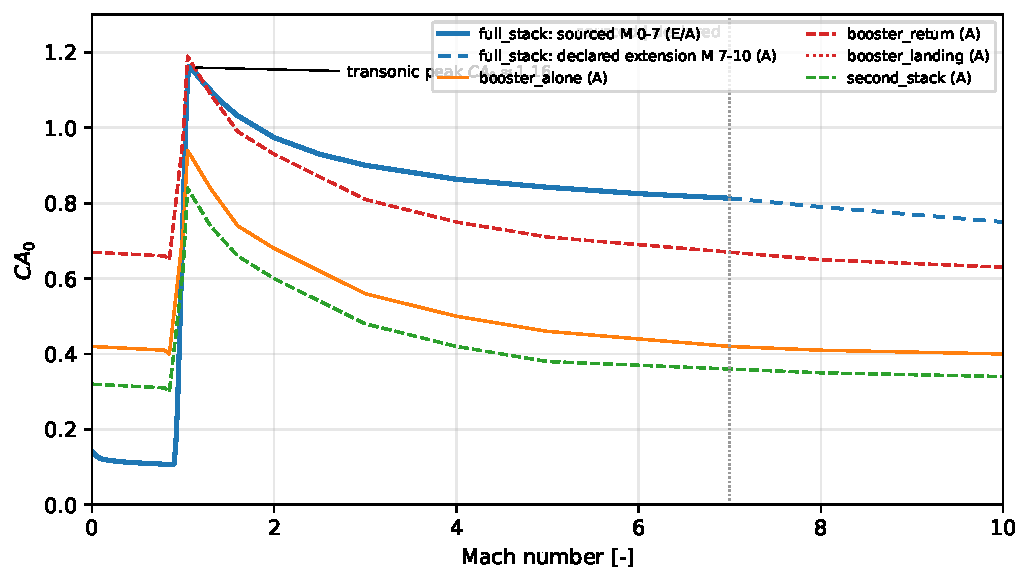
\includegraphics[width=0.85\linewidth]{images/aero_axial_curves.pdf}
\captionof{figure}{Axial drag coefficient $CA_0(M)$ of the five configurations.
Only the full-stack curve to Mach~7 is sourced; everything else is a
declared estimate (evidence classes in the legend). The transonic peak of
the full stack reaches $CA_0 \approx 1.16$.}
\label{fig:aero-axial-curves}
\end{minipage}\par\medskip

\subsection{Grid fin control}

The return/landing configurations have four fins at $45^\circ$, $135^\circ$, $225^\circ$ and $315^\circ$ about Body $+x$, station 39.6 m and pivot radius 1.83 m. Each uses area $1.65\,\mathrm{m^2}$, effective lift slope $1.2\,\mathrm{rad^{-1}}$ and travel $\pm0.35\,\mathrm{rad}$, all research-model assumptions. Equation~\eqref{eq:aero-fin} gives the force for deflection $\delta_i$ and azimuth $\varphi_i$:
\begin{equation}
 \vect F_i=\bar q S_{\mathrm{fin}}c_{\ell,\delta}\delta_i\cos\alpha|\cos\alpha|
 \begin{bmatrix}0&-\sin\varphi_i&\cos\varphi_i\end{bmatrix}^{\mathsf T}.
\label{eq:aero-fin}
\end{equation}
The three-dimensional mount arm generates pitch/yaw through axial offset and roll through radial offset. Equal deflections produce roll; differential pairs generate transverse moments. Command selection belongs to Section~\ref{sec:mission-exec}. The aerodynamic interface applies instantaneous deflections without servo dynamics. Mach/angle-dependent effectiveness, plume interference and deflection-induced axial drag are unresolved.

\subsection{Domain and verification}

The model rejects unsupported Mach values (the curves end at 10), unknown configurations, invalid stations and out-of-travel commands. Declared coefficient uncertainty remains an uncertainty within that domain, not an execution error.

The 42 aerodynamic tests check axial baselines, force direction, retro reversal, moment arms, dissipative damping, continuity, fin combinations and all configuration records, plus a short propagation through the dynamics provider. These checks verify the implementation; they do not validate the unsourced coefficient curves against flight data.
        % Ch 5
\section{Sensor Models and Measurement Generation}
\label{sec:sensors}

Four sensor front-ends generate measurements from the truth trajectory:
an \ac{IMU}, a \ac{GNSS} receiver, a \ac{LIDAR} altimeter, and a star
tracker (\texttt{sensors.py}). Sampling occurs only at accepted
integration times whose $0.01\,\mathrm{s}$ step is an integer multiple of
every sensor period, so all rates in Table~\ref{tab:sensors} are hit
exactly; no random numbers are drawn during integration trial
evaluations, and a fixed seed reproduces a run sample for sample. The
navigation-consumer side of these streams is the filter of
Section~\ref{sec:navigation}; this section covers measurement generation
only. All specs are placeholder research assumptions (classes A/C), not
certified Falcon~9 hardware.

\begin{table}[htbp]
\centering
\begin{tabular}{lllp{6.6cm}}
\toprule
Sensor & Rate & Mounting & Error model \\
\midrule
IMU & $100\,\mathrm{Hz}$ & station $[38,0,0]$ &
accel $\sigma = 0.01\,\mathrm{m/s^2}$, bias $[0.05,-0.03,0.02]\,\mathrm{m/s^2}$,
scale factor $10^{-3}$, bias random walk $10^{-4}$;
gyro $\sigma = 10^{-4}\,\mathrm{rad/s}$, bias $[0,0,10^{-4}]\,\mathrm{rad/s}$;
misalignment and temperature models supported \\
GNSS & $10\,\mathrm{Hz}$ & antenna $[41,0,0]$ &
pos $\sigma = [1.5, 1.5, 2.5]\,\mathrm{m}$ plus Gauss-Markov
$\sigma = [0.6, 0.6, 1.0]\,\mathrm{m}$ at $\tau = 300\,\mathrm{s}$;
vel $\sigma = 0.1\,\mathrm{m/s}$;
latency $0.1\,\mathrm{s}$; outages and dropouts supported \\
LiDAR & $10\,\mathrm{Hz}$ & station $[0.5,0,0]$, boresight $-x$ &
slant range $1$--$1\,800\,\mathrm{m}$,
$\sigma = 0.05\,\mathrm{m} + 10^{-4}\,R$ \\
Star tracker & $4\,\mathrm{Hz}$ & boresight $60^{\circ}$ from $+x$ toward $+y$ &
cross-boresight $\sigma = 5\,\mathrm{arcsec}$, boresight roll
$\sigma = 40\,\mathrm{arcsec}$; latency $0.1\,\mathrm{s}$ \\
\bottomrule
\end{tabular}
\caption{Sensor front-ends and adopted settings; the stations are Body
coordinates. Every entry is a placeholder research assumption (class A/C),
not a certified Falcon~9 sensor.}
\label{tab:sensors}
\end{table}

\subsection{Inertial measurement unit}

The \ac{IMU} measures specific force and angular rate at its fixed
structural station. The ideal specific force includes the station
kinematics of the dynamics core --- the angular-rate and
center-of-gravity-migration terms of moving the measurement point off the
center of gravity --- so the accelerometer senses what a real strapped-down
unit at that station would sense. Per sample, the measured pair is
%
\begin{equation}
\label{eq:imu-model}
\mathbf{f}_{\mathrm{meas}} = \mathbf{A}\,\mathbf{f}_{\mathrm{true}}
+ \mathbf{b}_a + \mathbf{b}_{a,T} + \mathbf{b}_{a,\mathrm{rw}} + \mathbf{n}_a,
\qquad
\boldsymbol{\omega}_{\mathrm{meas}} = \mathbf{G}\,\boldsymbol{\omega}_{\mathrm{true}}
+ \mathbf{b}_g + \mathbf{n}_g,
\end{equation}
%
with per-axis scale-factor/misalignment matrices
$\mathbf{A},\mathbf{G} = \mathbf{I} + \mathrm{diag}(\cdot) + \mathbf{M}$
(zero diagonal of $\mathbf{M}$), constant biases, temperature coefficients
about a $20\,^{\circ}\mathrm{C}$ reference, bias random walks driven per
sample as $\mathcal{N}(0, \sigma_{\mathrm{rw}}^2\,\Delta t)$, and white
noise at the sigmas of Table~\ref{tab:sensors}. The nominal mission uses
the biases, scale factor and random walk listed in the table, with
misalignment, temperature and gyro scale-factor terms at zero (modeled
but switched off). The gyro measures the Body rate relative to the
rotating \ac{ECEF} frame, consistent with the quaternion transport
equation the navigation filter propagates.

\subsection{GNSS, LiDAR and star tracker}

The \ac{GNSS} receiver provides antenna position and velocity in the
external frame, transformed from the truth state with the full lever-arm
kinematics (antenna station minus \ac{IMU} station, angular-rate cross
term and center-of-gravity migration). A $0.1\,\mathrm{s}$ latency model
feeds a truth-side history buffer that is linearly interpolated at the
delayed epoch, so the emitted sample is a measurement of the past state,
not of the present one. The position error is a first-order Gauss-Markov
process beside the white noise (updating per sample with the configured
$300\,\mathrm{s}$ correlation time), modelling the slow, correlated
component absent from naive white-noise \ac{GNSS} error. First-fix delays,
scheduled outages and random dropouts are supported and reported through
a validity flag; the nominal run has none of them, and every sample is
valid.

The \ac{LIDAR} measures slant range to the spherical ground along its
$-x$ boresight. Validity is geometric: the analytic line--sphere
intersection must exist, point downward and land inside the declared
$1$--$1\,800\,\mathrm{m}$ envelope; invalid geometry is reported as an
invalid sample, never extrapolated. Range noise is
$0.05\,\mathrm{m} + 10^{-4}R$.

The star tracker provides absolute attitude as a sensor-frame-to-\ac{ECI}
quaternion. The \ac{ECI} frame is defined to coincide with the
launch-aligned \ac{ECEF} frame at $t = 0$, and the Earth rotation carries
the conversion, so the injection of rotation into the attitude chain is
explicit rather than implicit. Noise is $5\,\mathrm{arcsec}$
cross-boresight and $40\,\mathrm{arcsec}$ about the boresight per
exposure, with a $0.1\,\mathrm{s}$ latency applied on the attitude
history. Availability is physical: the unit is blinded above
$2^{\circ}/\mathrm{s}$ body rate, below $60\,\mathrm{km}$ altitude
(dense atmosphere), inside the $20^{\circ}$ Earth-limb exclusion, and
optionally inside a $40^{\circ}$ solar exclusion; first-fix, outage and
dropout faults are supported (nominally off). The reported sample always
carries its blinding reason, making the availability record auditable in
the run output.

\paragraph*{Assumptions and limitations}
All noise, bias and latency values are declared placeholders, not datasheet
values; the \ac{GNSS} model has no ionospheric, tropospheric or multipath
terms; the \ac{LIDAR} assumes the bare sphere of
Section~\ref{sec:environment} as ground; the star tracker mounting is a
placeholder that keeps the boresight sky-pointing for an upright vehicle,
and vehicle-generated obscuration (plumes, stage interfaces) is not
modeled.
       % Ch 6
\section{Navigation Architecture and State Estimation}
\label{sec:navigation}

The navigation filter, \texttt{kalman.py}, is a multiplicative
error-state \ac{MEKF}: inertial prediction on the \ac{IMU} stream,
corrected by the \ac{GNSS}, \ac{LIDAR} and star-tracker measurements of
Section~\ref{sec:sensors}. The estimated state is referenced to the \ac{IMU}
station --- its position and velocity in the external frame --- so the
lever arms of the other sensors are constant Body vectors and no state
re-referencing occurs when the center of gravity migrates during burn.
The nominal 24-state configuration is
$\mathbf{x} = [\mathbf{p}, \mathbf{v}, \mathbf{b}_a,\,
\mathbf{q}, \mathbf{b}_g,\, \mathbf{s}_f,\, \mathbf{m}]$:
\ac{IMU}-station position and velocity, accelerometer bias, the attitude
quaternion from Body to \ac{ECEF} (Hamilton, scalar-first), gyro bias,
per-axis gyro scale factor and the six off-diagonal gyro misalignment
terms (Table~\ref{tab:nav-state}).

\begin{table}[htbp]
\centering
\begin{tabular}{lll}
\toprule
Block & Content & Initial $1\sigma$ \\
\midrule
$\mathbf{p}$, $\mathbf{v}$ & \ac{IMU}-station position, velocity [\textrm{m}, \textrm{m/s}] & $2\,\mathrm{m}$, $0.05\,\mathrm{m/s}$ \\
$\mathbf{b}_a$ & accelerometer bias, Body [$\mathrm{m/s^2}$] & $0.1$ \\
$\mathbf{q}$ & attitude (multiplicative error $\delta\boldsymbol{\theta}$, Body [rad]) & $0.01\,\mathrm{rad}$ \\
$\mathbf{b}_g$ & gyro bias, Body [$\mathrm{rad/s}$] & $10^{-3}$ \\
$\mathbf{s}_f$, $\mathbf{m}$ & gyro scale factor, misalignment & $10^{-3}$ \\
\bottomrule
\end{tabular}
\caption{Estimated-state blocks and initial standard deviations. The
initial position error is a seeded $[1, -1, 0.5]\,\mathrm{m}$; the attitude
starts at truth with a $0.01\,\mathrm{rad}$ prior unless declared
otherwise.}
\label{tab:nav-state}
\end{table}

\subsection{Prediction}

Each $100\,\mathrm{Hz}$ \ac{IMU} sample advances the strapdown state. The
gyro measurement is corrected with the current calibration estimate,
$\hat{\boldsymbol{\omega}} = \hat{\mathbf{G}}^{-1}
(\boldsymbol{\omega}_{\mathrm{meas}} - \hat{\mathbf{b}}_g)$, and the
attitude is propagated by its quaternion transport equation with the
trapezoidal mean rate over the interval; the mid-interval attitude
rotates the bias-corrected specific force into the external frame
alongside the modelled gravity and rotating-frame accelerations of
Section~\ref{sec:environment}, whose analytical gradients linearize that
model in the filter. The error dynamics couple the multiplicative attitude
error into the velocity error through $-\mathbf{R}\,[\hat{\mathbf{f}}]_\times
\delta\boldsymbol{\theta}$, and the gyro chain drives the attitude error
through the bias, scale-factor and misalignment blocks --- the calibration
is observable only through attitude aiding and sufficient angular motion.
Process noise is built from the sensor \acp{PSD}
($\sigma_a^2/f_{\mathrm{IMU}}$, $\sigma_g^2/f_{\mathrm{IMU}}$) and the
declared bias random walks.

\subsection{Measurement updates}

All corrections use the Joseph-form covariance update and record a
normalized innovation square for monitoring. The \ac{GNSS} update corrects
position and velocity: its $0.1\,\mathrm{s}$ latency is compensated by
extrapolating the measurement to the current epoch with the estimated
acceleration, its lever arm (antenna minus \ac{IMU} station) is removed
with the angular rate, and the measurement Jacobian carries the full
attitude, bias and calibration sensitivity of that arm. The \ac{LIDAR}
update is scalar and nonlinear: the measurement is the analytic
line--sphere slant range of Section~\ref{sec:sensors}, differentiated
analytically at the estimated state, with attitude sensitivity through
both the arm and the boresight direction; invalid geometry skips the
update. The star-tracker update is an absolute attitude correction: the
measurement quaternion is converted from \ac{ECI} to \ac{ECEF} by the
Earth rotation at the exposure epoch, propagated over its latency with
the last estimated body rate, and differenced multiplicatively from the
estimated attitude; its noise covariance is rotated into the Body frame by
the known mounting, and the update is gated by the three-degree-of-freedom
\ac{NIS} at the $99.9\,\%$ level ($16.27$), with rejects counted rather
than silently absorbed.

\subsection{Interfaces and diagnostics}

The filter consumes its own attitude estimate by default
(\texttt{use\_estimated\_attitude}): the prediction rotates the specific
force with the estimated quaternion, and every GNSS, \ac{LIDAR} and
star-tracker correction also corrects that attitude. A declared
diagnostic mode retains the original nine-state filter with the truth
attitude supplied from outside; its results are kept distinct from the
gyro-driven results in the results chapter. A second, deliberately
unaided baseline propagates the attitude from the raw gyro stream alone
(\texttt{GyroAttitude}): starting from the same initial attitude, it
carries uncompensated gyro noise and bias, and its logged error isolates
how much the aiding buys over pure dead reckoning. One filter instance
runs across staging without a reset --- the estimated state is
\ac{IMU}-station referenced and the sensor stations are stage-1
hardware, so the booster return needs no state handover; the separated
upper stage flies an open-loop truth continuation without a navigation
instance.

\subsection{Verification and nominal-run behavior}

The filter is verified in stages: numeric finite-difference checks confirm
the analytic Jacobians of the attitude error with respect to gyro bias,
scale factor and misalignment; a closed-loop scenario (a vehicle
exercised on the rotating Earth with star-tracker aiding) recovers
injected bias, scale-factor and misalignment values; and the cross-module
and mission-level suites (115 tests, all green) exercise the integrated
chain end to end. In the nominal full-mission run the filter operates in
its default gyro-driven configuration: the position error holds
$0.881\,\mathrm{m}$ \ac{RMS} ($0.918\,\mathrm{m}$ in the truth-attitude
reference configuration), the aided attitude error stays at
$0.456^{\circ}$ \ac{RMS} (peak $1.57^{\circ}$, touchdown
$0.012^{\circ}$) while the unaided gyro baseline drifts monotonically to
$1.89^{\circ}$, and the $z$-axis gyro bias is recovered to $1.4\,\%$.
The \ac{GNSS} innovations are statistically consistent (mean \ac{NIS}
$7.58$ for six degrees of freedom) and \ac{LIDAR} delivers $496$ valid
updates. All $381$ valid star-tracker exposures are rejected by the
\ac{NIS} gate: the propagated attitude uncertainty ($1\sigma$ median
$0.118^{\circ}$) understates the actual maneuver-induced error by more
than the factor the $99.9\,\%$ gate tolerates, so the nominal attitude is
gyro-propagated with weak \ac{GNSS} lever-arm aiding only --- the gate
outcome and its causes are treated as a result in the results chapter of
this report.

\paragraph*{Assumptions and limitations}
All noise and bias parameters are the placeholder research assumptions of
Table~\ref{tab:sensors}; the gyro calibration block estimates a unit whose
adopted true misalignment and scale factor are zero, so its output is a
zero-check rather than a calibration demo; \ac{GNSS} latency compensation
assumes constant acceleration across the $0.1\,\mathrm{s}$ window;
attitude prior and initialization are declared values, not surveyed
alignment; and the filter has no protection against unmodeled faults
beyond the star-tracker \ac{NIS} gate --- every update it accepts is
trusted once inside the gate.
          % Ch 7
\section{Ascent, Staging and Upper Stage}
\label{sec:ascent}

This chapter describes the command laws behind the mission phases of
Section~\ref{sec:vehicle}: the ascent attitude program, the engine
shutdown, the separation state map with its audit, and the separated
upper-stage continuation. The event machine, step control and state bookkeeping of the run loop are
described in the architecture chapter of this report.

\subsection{Attitude program and ascent control}

Powered ascent flies a pitch program with an ideal attitude-control law.
The commanded tilt grows from vertical along
%
\begin{equation}
\label{eq:pitch-program}
\theta(t) = \theta_{\max}\,
\frac{x^2}{1+x^2},
\qquad x = \frac{t - t_s}{\tau},
\end{equation}
%
with $t_s = 8\,\mathrm{s}$, $\tau = 100\,\mathrm{s}$ and
$\theta_{\max} = 80^{\circ}$ toward a $45^{\circ}$ north-east heading (an
\ac{ISS}-launch approximation). The tilt law is calibrated against the
video-derived ascent reference used in the results chapter; it is not
independently validated guidance (class A). Attitude tracking applies a
proportional-derivative law on the Body-frame attitude error
$\mathbf{e}$ and angular rate,
%
\begin{equation}
\label{eq:attitude-pd}
\boldsymbol{\alpha} = k_p\,\mathbf{e} - k_d\,\boldsymbol{\omega},
\qquad
\mathbf{M} = \mathbf{J}\,\boldsymbol{\alpha},
\quad k_p = 2.0,\; k_d = 2.5,
\end{equation}
%
an unlimited ideal moment: the ascent controller relies on the
actuation chain only for realistic execution, and the provider optionally
enforces a declared angle-of-attack limit, raising a domain error when the
flight exceeds it.

\subsection{Engine shutdown and event guards}

Engine cutoff at $140\,\mathrm{s}$ follows a quintic flow envelope, not an
instantaneous stop:
%
\begin{equation}
\label{eq:quintic-shutdown}
\gamma(u) = (1-u)^3 (1 + 3u + 6u^2),
\qquad
\gamma'(u) = -\,\frac{30\,u^2 (1-u)^2}{T},
\quad u = \frac{t - t_0}{T},
\end{equation}
%
with $T = 1\,\mathrm{s}$ and completion anchored to the published
$141\,\mathrm{s}$ MECO reference. The envelope and its derivative are
supplied together to the integrator, keeping mass flow and flow rate
consistent during the ramp; the duration is a numerical design choice of
class A, anchored to, not measured from, the reference
timeline. Event transitions carry guards that must hold at the event:
separation requires zero flow, engines off and the full stack attached;
boostback, entry and landing ignitions additionally require the
respective propellant budget (including the reserve),
attitude readiness and propulsion readiness, and for the latter two a
descending trajectory. Each burn ends through a smooth ramp with its own
reason: predicted-miss tolerance, speed target, or budget cap.

\subsection{Stage separation and conservation audit}

Separation at $144\,\mathrm{s}$ is a zero-impulse, no-discard state map:
the coasting parent is split into booster and upper stack at the
stage-2 interface, both children keep the parent attitude and angular
rate, and the upper stage's stations are renumbered to its own aft-skirt
datum. The map refuses to run while any engine command or flow is active,
and its result is only returned if a conservation audit confirms
continuity to tight tolerances: mass, linear momentum, angular momentum
about the Earth-centred origin and kinetic energy are conserved to
$10^{-10}$ relative residual, fixed structural points keep their
ECEF position and velocity to $10^{-8}\,\mathrm{m/m/s}$, and attitude and
angular rate are preserved to $10^{-12}$. The audit quantities (all
residuals, and both child masses) are recorded in the run's event record,
and the results chapter quotes them.

\subsection{Upper-stage continuation}

After separation the upper stack continues under its own reduced provider
as a six-degree-of-freedom propagation from the conserved separation
state: a single MVac engine at $0.95$ throttle with quintic ignition and
cutoff ramps (the standard $10u^3 - 15u^4 + 6u^5$ envelope) over
$1\,\mathrm{s}$ at $152\,\mathrm{s}$ ignition and $545\,\mathrm{s}$
cutoff, an attitude law of the form of Equation~\eqref{eq:attitude-pd}
($k_p = 2.0$, $k_d = 2.5$) holding the separation heading, and a simple
axial-drag estimate of $C_D = 0.3$ on the $10.52\,\mathrm{m^2}$ stage
cross-section --- deliberately not the declared \texttt{second\_stack}
aerodynamic configuration of Section~\ref{sec:aero}. These are
demonstration commands of class A, not reconstructed flight data: the
continuation exists to show the separated state and the conserved
separation map, and its SECO state (about $200\,\mathrm{km}$ altitude at
$1\,600\,\mathrm{km}$ surface distance in the nominal run) feeds the
flight-path overview of Figure~\ref{fig:flightpaths} rather than any
orbital-accuracy claim.
      % Ch 8 material - to be merged into content/mission_execution.tex
\section{Booster Return, Control and Actuation}
\label{sec:return}

The return controller commands the separated booster from separation to
touchdown through the phases of Section~\ref{sec:vehicle}: boostback
burn, return coast, entry burn, aerodynamic descent and landing burn
(\texttt{recovery.py}). Control is recomputed on a fixed
guidance period of $0.2\,\mathrm{s}$; throttle changes run through
$1\,\mathrm{s}$ smooth ramps, and the burn timing of the nominal run
appears in Figure~\ref{fig:thrust-profile}. Boostback and entry burns
run the three-engine set $(0,1,5)$; the landing burn runs the single
center engine. The legs deploy at landing ignition. The
controller feeds back the truth state and commands ideal attitude
moments --- class A project assumptions --- so the navigation solution is
deliberately not in the loop yet.

\begin{figure}[htbp]
\centering
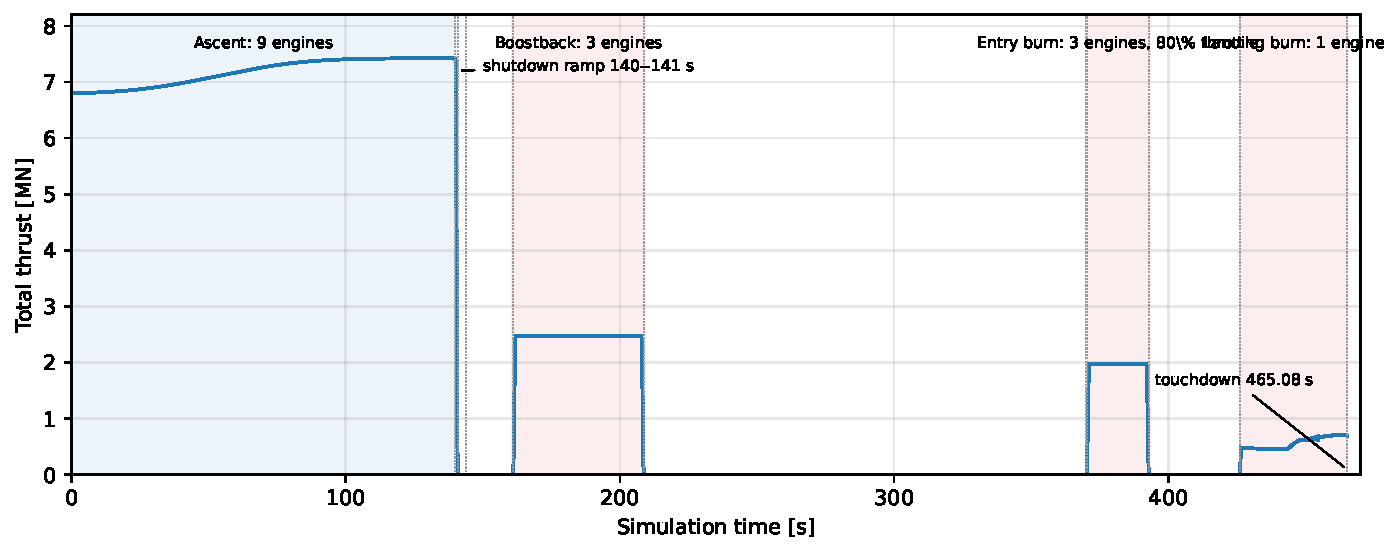
\includegraphics[width=\linewidth]{images/thrust_profile.pdf}
\caption{Total thrust of the nominal full-mission run (seed 1). The
booster burns are command-planned: boostback on three engines at full
throttle, the entry burn on three engines at $80\,\%$ throttle, and the
landing burn on the single center engine. Touchdown at
$t = 465.08\,\mathrm{s}$.}
\label{fig:thrust-profile}
\end{figure}

\subsection{Boostback: prediction and steering}

Boostback steering inverts a predicted landing miss. A reduced-order
ballistic predictor propagates the booster state forward in
$0.5\,\mathrm{s}$ steps with central gravity and rotating-frame
accelerations (Section~\ref{sec:environment}), the declared
\texttt{booster\_return} axial and crossflow coefficients
(Section~\ref{sec:aero}), and a prospective three-engine entry burn at the
declared altitude and throttle; the resulting predicted impact miss is
refreshed every second. During coast and the burn, the commanded
acceleration is
%
\begin{equation}
\label{eq:boostback-law}
\mathbf{a}_{\mathrm{cmd}} = -\,\frac{\hat{\mathbf{m}}}{8\,t_f}
\;+\; 0.8\,\hat{\mathbf{u}},
\end{equation}
%
where $\hat{\mathbf{m}}$ is the predicted miss vector, $t_f$ the ballistic
flight time and $\hat{\mathbf{u}}$ the local vertical. The burn stops on
the first satisfied condition: the predicted miss norm falls below
$500\,\mathrm{m}$ (the "predicted ballistic miss tolerance"), or the
burn duration leaves its $10$--$60\,\mathrm{s}$ planning window, or its
budget cap is reached. In the nominal run the boostback ends at
$208.81\,\mathrm{s}$ on the planning cap.

\subsection{Entry burn and aerodynamic descent}

Entry ignition requires the descending-through-$45\,\mathrm{km}$
condition plus the restart guards (budget, attitude, propulsion). During
the burn the commanded acceleration is a $30\,\mathrm{m/s^2}$ retrograde
bias plus lateral correction,
$\mathbf{a}_{\mathrm{cmd}} = 30\,\hat{\mathbf{u}} +
(\mathbf{v}_{d,h} - \mathbf{v}_h)/8 - \mathbf{a}_{\mathrm{aero}}$, toward
the desired horizontal velocity
$\mathbf{v}_{d,h} = -\mathbf{e}_h/(t_f + 25\,\mathrm{s})$ that nulls the
target error over the remaining flight. The burn ends when the speed
reaches $500\,\mathrm{m/s}$ or its budget cap fires. Through the
aerodynamic descent the vehicle holds a retrograde attitude above
$8\,\mathrm{km}$ and transitions to vertical attitude below, with the
grid fins available for residual moment demand.

\subsection{Landing burn and touchdown}

Landing ignition is predictive: a reduced-order stopping simulation
propagates the booster in $0.1\,\mathrm{s}$ steps with the landing
aerodynamic model, tilted thrust scaled by the ignition factor $1.05$,
and the current throttle amplitude; when the simulated stop leaves the
vehicle no more than the declared $1.5\,\mathrm{km}$ clearance allowance
above the ground, the burn ignites (nominal: $426.16\,\mathrm{s}$). The
guidance law is a second-order polynomial descent to the target with
terminal vertical velocity $v_{t} = -0.5\,\mathrm{m/s}$:
%
\begin{equation}
\label{eq:landing-law}
\mathbf{a}_{\mathrm{cmd}} = \frac{6\,(\mathbf{r}_{\mathrm{goal}} -
\mathbf{r})}{t_{go}^2} - \frac{4\,\mathbf{v}}{t_{go}}
- \frac{2\,v_t}{t_{go}}\,\hat{\mathbf{u}}
- \mathbf{g} - \mathbf{a}_{\mathrm{aero}},
\end{equation}
%
with $t_{go}$ from the current altitude and sink rate. The lateral
component of Equation~\eqref{eq:landing-law} is clamped by the
$20^{\circ}$ tilt limit, which tapers to a $4^{\circ}$ terminal attitude
below the $20\,\mathrm{m}$ hold height. Touchdown is the ground contact
of the lowest leg tip --- four assumed tips, $1\,\mathrm{m}$ below the
base at a $3.5\,\mathrm{m}$ radius --- and the run loop resolves the
contact instant by bisection; the acceptance criteria of
Table~\ref{tab:landing-limits} are evaluated at that instant. The
command path from guidance through actuation to the applied forces and
moments is completed by the actuator layer.

\begin{table}[htbp]
\centering
\begin{tabular}{lrr}
\toprule
Landing acceptance metric & Limit & Result (nominal run) \\
\midrule
Vertical speed & $\le 2\,\mathrm{m/s}$ & $0.497\,\mathrm{m/s}$ \\
Horizontal speed & $\le 1\,\mathrm{m/s}$ & $0.902\,\mathrm{m/s}$ \\
Target error & $\le 10\,\mathrm{m}$ & $3.306\,\mathrm{m}$ \\
Tilt & $\le 5^{\circ}$ & $0.535^{\circ}$ \\
Angular rate & $\le 1\,^{\circ}/\mathrm{s}$ & $0.013\,^{\circ}/\mathrm{s}$ \\
\bottomrule
\end{tabular}
\caption{Provisional project acceptance limits for a near-stationary
upright contact (class A; not Falcon~9 certified limits) and the nominal
run's contact metrics at $465.083\,\mathrm{s}$.}
\label{tab:landing-limits}
\end{table}

\subsection{Force and moment allocation}

Each commanded acceleration is converted to a bounded force allocation:
a numerical solver chooses the nose direction within the active tilt
envelope, the engine count and the throttle such that the resultant of
engine thrust (vacuum thrust minus exit-area ambient pressure at the
engine station) and the modelled aerodynamic reaction matches the
requested force; the corresponding ideal attitude moment drives the
vehicle toward that nose direction, with the moment authority capped at
$2\,\mathrm{MN\,m}$ during burns and $200\,\mathrm{kN\,m}$ in coast. Grid
fins carry residual moment demand beyond the virtual-vector authority,
mainly roll. Control gains: attitude $k_p = 1.0$,
$k_d = 2.0$; landing lateral $k_p = 0.0576$, $k_d = 0.48$; landing
attitude $k_p = 1.5$, $k_d = 6.0$.

% +++++ PENDING SUBSECTION (see ../docs/flags.md FL-2): Actuator layer.
% To be written LAST, against the final Actuators.py implementation:
% command path from the recovery/attitude laws through actuator dynamics
% to TVC gimbal (5 deg limit) and grid-fin rate/travel (+/-20 deg)
% forces and moments, ramp/rate limits, and its tests. Ground every
% statement in the implemented code; scope to what exists; then re-run
% the test suites, re-generate the nominal run and update
% Figure~\ref{fig:thrust-profile} if behavior changed.
      % Ch 8 material - to be merged into content/mission_execution.tex;
                                   %   results blocks (thrust profile, landing table) move to Ch 9
%\section{Verification, Validation, and Simulation Results}
\label{sec:results}

This chapter separates verification of implemented equations, comparison with public flight evidence, and navigation error against simulation truth. The final nominal record R1 uses seed 1, $0.01\,\mathrm{s}$ maximum step, 100 Hz IMU and $0.1\,\mathrm{s}$ output; its original path is given in Appendix~\ref{sec:appendix-reproduction}. All 31 runtime/data fingerprints match the reviewed source. The shared archive and \path{report/reproduce.py} regenerate the result panels and numerical macros without another full-flight integration. The provenance ledger \path{report/figure_sources.json} records source hashes and extracted metrics.

\subsection{Model verification and state continuity}
The vehicle/navigation suite contains 130 passing assertion-based tests; the environment suite adds 41. They cover mass aggregation and derivatives, force-arm signs, fixed-mass free fall and constant-moment rotation, rotating Body storage, propellant bounds, aerodynamic flow reversal/damping, event guards, separation and two-child execution. Navigation tests add tolerance-based finite differences for the 30-state transition, SO(3) right Jacobian and sensor sensitivities, as well as startup epoch, delayed-attitude, gate and colored-noise checks. The legacy print-only diagnostics are not counted as assertion tests. These checks establish behavior in their fixtures, rather than agreement with real hardware.

At $144\,\mathrm{s}$, parent mass is $211019.374\,\mathrm{kg}$ and child masses are $91089.374$ and $119930.000\,\mathrm{kg}$. Their mass residual is zero. Relative linear- and angular-momentum residuals are $9.95\times10^{-19}$ and $9.54\times10^{-12}$; recombined-CG position error is $4.66\times10^{-10}\,\mathrm{m}$. These satisfy the numerical criteria of Section~\ref{sec:vehicle} for the assumed zero-impulse map. Both child states remain finite and are propagated without replacing their inherited initial conditions. Conservation under an assumed map does not establish the accuracy of real separation impulses or discarded hardware.

\subsection{Continuous mission and separated trajectories}
Figure~\ref{fig:results-flight} shows the complete generated sequence, and Figure~\ref{fig:results-trajectories} distinguishes the two children. Shutdown completes at 141 and separation occurs at $144\,\mathrm{s}$. The three return burns and their measured consumption appear in Table~\ref{tab:burn-results}; their endpoints are integration results of the conditions in Section~\ref{sec:mission-exec}.

\par\medskip\noindent\begin{minipage}{\linewidth}
\centering
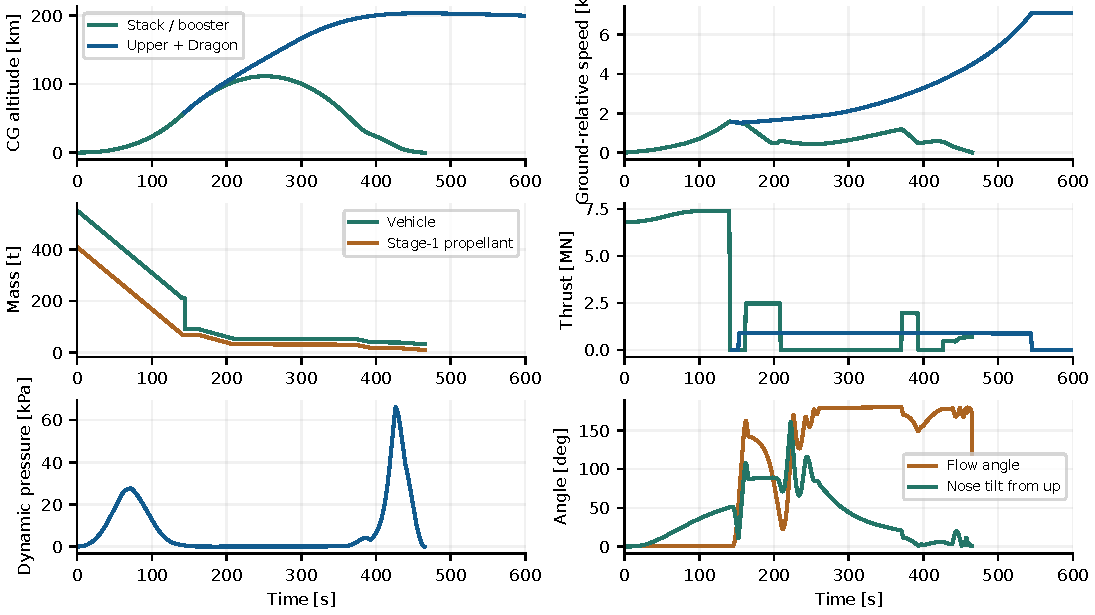
\includegraphics[width=\linewidth]{images/results_flight_profiles.pdf}
\captionof{figure}{R1 continuous flight. Green denotes stack/booster and blue the upper child where both are shown. The mass jump is a change of tracked configuration at separation. Flow angle near $180^\circ$ means engine-first relative flow, not attitude-estimation error. The trajectories use project commands and truth-state feedback.}
\label{fig:results-flight}
\end{minipage}\par\medskip

\par\medskip\noindent\begin{minipage}{\linewidth}
\centering\small
\begin{tabular}{@{}lrrl@{}}
\toprule
Burn & Start--end [s] & Consumed [t] & End condition \\
\midrule
Boostback & 161.00--208.81 & 37.982 & Fuel/duration planning cap \\
Entry & 370.14--392.95 & 14.158 & Speed target, then smooth shutdown \\
Landing & 426.16--465.083 & 7.818 & First contact \\
\bottomrule
\end{tabular}
\captionof{table}{Observed R1 return-burn intervals and fuel consumption. Boostback reaches its planning cap rather than the 500 m predicted-miss target. Its recorded predicted miss at burn end is about 3.97 km; later phases provide additional correction.}
\label{tab:burn-results}
\end{minipage}\par\medskip

The ascent dynamic-pressure maximum is $27.62\,\mathrm{kPa}$ at $71.9\,\mathrm{s}$, compared with the approximate $75\,\mathrm{s}$ preflight marker. The full-flight maximum is instead $66.16\,\mathrm{kPa}$ near landing ignition at $426.3\,\mathrm{s}$; the two maxima must not be confused. Between entry shutdown and landing ignition, gravity accelerates the unpowered descending booster again, explaining the late rise in its speed. Landing then brakes it to the contact state.

\par\medskip\noindent\begin{minipage}{\linewidth}
\centering
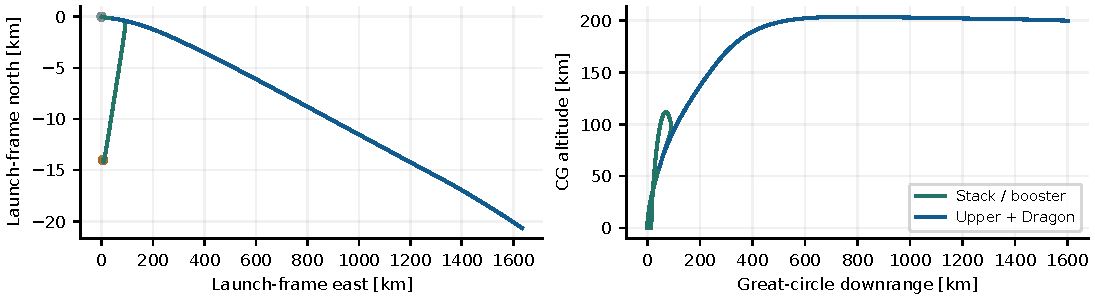
\includegraphics[width=\linewidth]{images/results_trajectories.pdf}
\captionof{figure}{R1 separated paths: launch-frame horizontal projection and altitude against spherical downrange. The marked horizontal points are launch and the assumed return target. The booster returns while the upper-stage/Dragon child continues downrange from the same separation event.}
\label{fig:results-trajectories}
\end{minipage}\par\medskip

Figure~\ref{fig:results-kinematics} completes the kinematic outputs requested in the assignment \cite[slide 5]{project2}. Great-circle downrange is $R_E\arccos(\hat{\vect r}\cdot\hat{\vect r}_{\mathrm{pad}})$; it is distance from the pad, not accumulated path length. Flight-path angle is $\gamma=\operatorname{atan2}(v_r,\lVert\vect v-v_r\hat{\vect r}\rVert)$, where $v_r=\vect v\cdot\hat{\vect r}$ and $\vect v$ is CG Earth-relative velocity. Actual rate magnitude peaks at $17.825^\circ\,\mathrm{s^{-1}}$ at $223.7\,\mathrm{s}$ in return coast. This is compatible with the per-axis desired-rate clip of Section~\ref{sec:mission-exec}; it is not a state-norm limit.

\par\medskip\noindent\begin{minipage}{\linewidth}
\centering
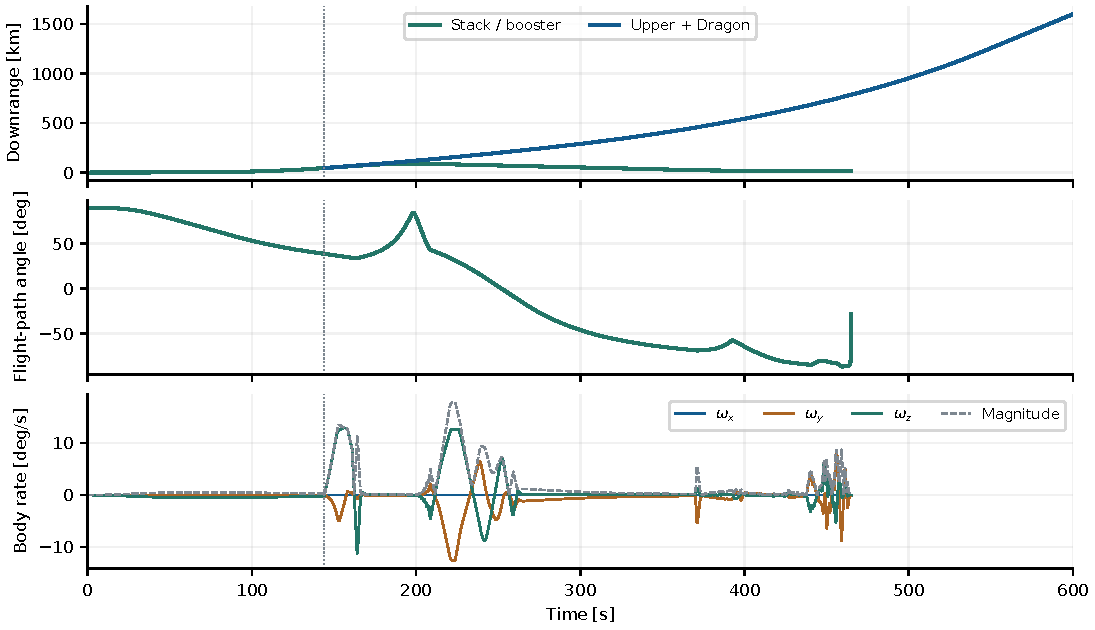
\includegraphics[width=\linewidth]{images/results_kinematics.pdf}
\captionof{figure}{R1 downrange for both children, stack/booster flight-path angle, and true Body-rate components/magnitude. Positive flight-path angle denotes outward motion; negative denotes descent. The angle is omitted below $1\,\mathrm{m\,s^{-1}}$, where direction is poorly defined. The dotted line marks separation. The post-boostback coast turn explains the largest rate excursion.}
\label{fig:results-kinematics}
\end{minipage}\par\medskip

Table~\ref{tab:landing-results} evaluates the project limits at contact. Contact occurs at $465.0827\,\mathrm{s}$ with $8.931\,\mathrm{t}$ of stage-1 propellant remaining. The ground condition applies to the lowest leg tip, so the CG remains above zero altitude. The upper child continues to $600\,\mathrm{s}$, reaching $199.694\,\mathrm{km}$ and $7.097\,\mathrm{km\,s^{-1}}$, with $5.472\,\mathrm{t}$ of propellant. This is a successful project scenario, not proof of SpaceX guidance reconstruction or validated orbital insertion.

\par\medskip\noindent\begin{minipage}{\linewidth}
\centering\small
\begin{tabular}{@{}lrr@{}}
\toprule
Acceptance metric & R1 result & Project limit \\
\midrule
Vertical speed [$\mathrm{m\,s^{-1}}$] & 0.4975 & 2 \\
Horizontal speed [$\mathrm{m\,s^{-1}}$] & 0.9016 & 1 \\
Tilt [deg] & 0.5349 & 5 \\
Angular-rate magnitude [$\mathrm{deg\,s^{-1}}$] & 0.01289 & 1 \\
Horizontal target error [m] & 3.306 & 10 \\
\bottomrule
\end{tabular}
\captionof{table}{R1 mission-level contact metrics. Speeds and target error use the structural-base state; ground contact is tested at the lowest leg tip. Ground contact and deployed legs are also required and satisfied. These are assumed project limits; horizontal speed has the smallest fractional margin.}
\label{tab:landing-results}
\end{minipage}\par\medskip

\subsection{Comparison with the ascent reference}
\label{sec:ascent-results}
Figure~\ref{fig:results-reference} compares 140 retained video-derived samples over $0$--$139.973\,\mathrm{s}$ \cite{crs10webcast,crs10telemetry}. Altitude RMSE is $1.577\,\mathrm{km}$ and speed RMSE $18.46\,\mathrm{m\,s^{-1}}$. At the last sample, simulated altitude is $54.628\,\mathrm{km}$ versus $59.400\,\mathrm{km}$, a $-8.03\%$ difference; speed is $1574.19$ versus $1609.44\,\mathrm{m\,s^{-1}}$, a $-2.19\%$ difference.

\par\medskip\noindent\begin{minipage}{\linewidth}
\centering
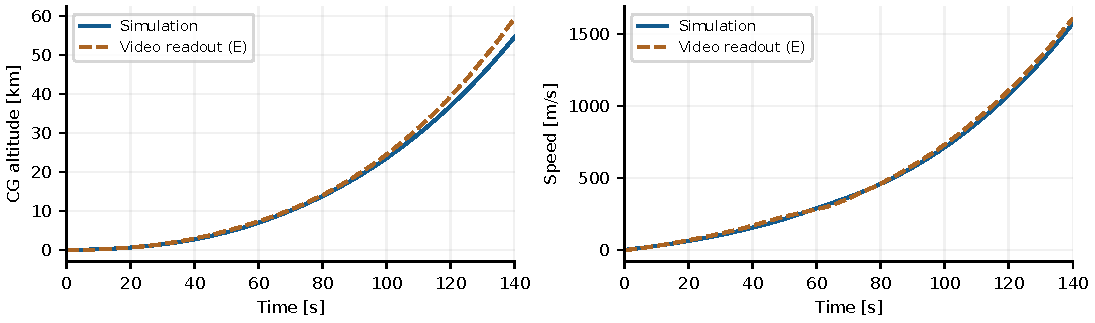
\includegraphics[width=\linewidth]{images/results_ascent_reference.pdf}
\captionof{figure}{R1 ascent against the E-class digitized broadcast readouts. This is the same record used to calibrate the ascent operating point/pitch timescale. Model CG altitude and ground-relative speed are compared with readouts whose detailed datum/frame conventions are not independently established.}
\label{fig:results-reference}
\end{minipage}\par\medskip

The comparison supports quantitative calibration within the retained ascent interval. It does not independently validate the tuned parameters, establish internal mass properties, or validate the return/upper-stage commands. Readout rounding, digitization and speed-frame uncertainty also limit interpretation of the residuals as pure physical-model error. The fairing-to-Dragon aerodynamic transfer and mixed-source vehicle data remain model uncertainties.

\subsection{Navigation accuracy and statistical diagnostics}
\label{sec:nav-results}
The gyro-driven navigation result is evaluated at the fixed IMU station, not at the moving CG. Equation~\eqref{eq:error-metrics} defines the three-dimensional position RMS and shortest quaternion-error angle used below:
\begin{equation}
 \mathrm{RMS}_p=\sqrt{\frac1N\sum_{k=1}^{N}\lVert\hat{\vect p}_k-\vect p_{\mathrm{true},k}\rVert^2},\qquad
 e_q=2\arccos\!\left(\left|\hat{\vect q}^{\mathsf T}\vect q_{\mathrm{true}}\right|\right).
\label{eq:error-metrics}
\end{equation}
The quaternion inner product is clamped numerically to $[0,1]$. Velocity RMS uses the corresponding velocity error. Figure~\ref{fig:results-navigation} shows accuracy and uncertainty diagnostics together.

\par\medskip\noindent\begin{minipage}{\linewidth}
\centering
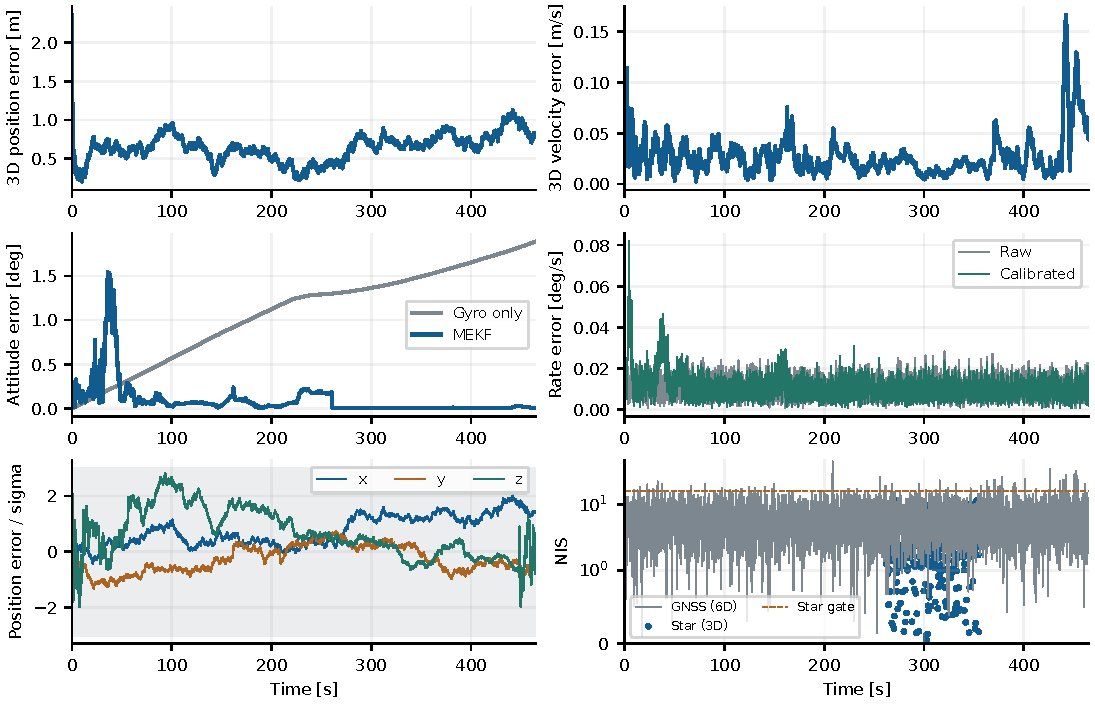
\includegraphics[width=\linewidth]{images/results_navigation.pdf}
\captionof{figure}{R1 navigation at the IMU station: position/velocity errors, estimated versus unaided attitude error, raw/calibrated angular-rate errors, normalized position errors and innovation diagnostics. The shaded interval is $\pm3$ reported standard deviations. The star gate is unchanged at 16.27; GNSS NIS is diagnostic. Accuracy, covariance consistency and rate calibration are assessed separately.}
\label{fig:results-navigation}
\end{minipage}\par\medskip

Position RMS is $\PositionRMS\,\mathrm{m}$, velocity RMS $\VelocityRMS\,\mathrm{m\,s^{-1}}$, and attitude RMS $\AttitudeRMS^\circ$. Attitude error peaks at $\AttitudePeak^\circ$ near $\AttitudePeakTime\,\mathrm{s}$ and ends at $\AttitudeFinal^\circ$, versus $\GyroOnlyFinal^\circ$ for the paired unaided gyro quaternion. These are simulation-truth errors under the declared alignment and sensor settings.

The archived earlier filter supplies a controlled comparison: both truth trajectories are byte-identical to R1 and all common raw sensor fields are identical sample by sample. Its position/velocity/attitude RMS values are $0.881\,\mathrm{m}$, $0.1354\,\mathrm{m\,s^{-1}}$ and $0.456^\circ$. The improvement measures the combined estimator changes of Section~\ref{sec:navigation}; it does not isolate each change's contribution. Physical flight and guidance are unchanged.

LiDAR supplies 496 valid corrections. All $\StarAccepted$ valid star exposures are accepted, with $\StarRejected$ rejected; the gate remains 16.27. Their mean and maximum NIS are $\StarNIS$ and $\StarMaxNIS$, and mean six-component GNSS NIS is $\GnssNIS$. Position errors remain inside reported $\pm3\sigma$ at every recorded epoch on all three axes. These correlated time samples are diagnostics, not independent coverage probabilities. All 4652 stored $30\times30$ covariance matrices are finite and symmetric, with minimum eigenvalue $1.01\times10^{-12}$; full matrices are archived for inspection.

Across $\RateSamples$ synchronized IMU/output epochs, calibrated angular-rate RMS is $\CalibratedRateRMS^\circ\,\mathrm{s^{-1}}$, compared with raw $\RawRateRMS^\circ\,\mathrm{s^{-1}}$. The nominal true gyro scale/cross-axis errors are zero; estimating them adds finite-sample uncertainty and does not guarantee improved instantaneous rates. The output remains an estimate of angular velocity, but this nominal case alone is insufficient evidence of calibration benefit. The independent nonzero-error test below supplies that evidence within its own excitation conditions.

\subsection{Independent navigation and covariance tests}
The executable \path{report/validate_navigation.py} supplies controlled truths independently of the CRS-10 trajectory. It runs a three-axis accelerometer-scale fixture, an analytic three-axis attitude fixture with nonzero gyro calibration errors, and 20 independent position/covariance realizations. Tolerances and fixture settings are explicit in Table~\ref{tab:independent-navigation} and Appendix~\ref{sec:appendix-reproduction}; all ten stored checks, including the isolated RK4 test below, pass. Figure~\ref{fig:independent-navigation} shows convergence and the independent final-epoch errors.

\par\medskip\noindent\begin{minipage}{\linewidth}
\centering\small
\begin{tabularx}{\linewidth}{@{}p{.34\linewidth}XX@{}}
\toprule
Independent check & Measured result & Acceptance criterion \\
\midrule
Accelerometer scale / bias error norm & $3.02\times10^{-5}$ / $3.79\times10^{-5}\,\mathrm{m\,s^{-2}}$ & $<4\times10^{-4}$ / $<0.002\,\mathrm{m\,s^{-2}}$ \\
Final attitude / gyro bias error norm & $0.00363^\circ$ / $1.21\times10^{-6}\,\mathrm{rad\,s^{-1}}$ & $<0.03^\circ$ / $<2\times10^{-5}\,\mathrm{rad\,s^{-1}}$ \\
Gyro scale / cross-axis error norm & $1.88\times10^{-4}$ / $8.06\times10^{-5}\,\mathrm{rad}$ & $<4\times10^{-4}$ / $<8\times10^{-4}\,\mathrm{rad}$ \\
Late-window raw / calibrated rate RMS & $0.03751/0.01004^\circ\,\mathrm{s^{-1}}$ & Calibrated RMS smaller \\
Position ANEES, 20 independent trials & $2.377$ (3 coordinates) & 95\% interval $[2.024,4.165]$ \\
GNSS mean NIS in the same fixture & $5.957$ (6 components) & Engineering check $5.5$--$6.5$ \\
\bottomrule
\end{tabularx}
\captionof{table}{Independent navigation checks. Error norms compare estimated parameters with injected truth. Numerical calibration tolerances and the NIS band are chosen engineering criteria; the ANEES interval has a stated chi-square statistical interpretation.}
\label{tab:independent-navigation}
\end{minipage}\par\medskip

For $M=20$ independent final position errors, $\mathrm{ANEES}=M^{-1}\sum_i\vect e_i^{\mathsf T}\mat P_{p,i}^{-1}\vect e_i$. The nominal 95\% acceptance interval is $[\chi^2_{60,0.025},\chi^2_{60,0.975}]/20$ \cite{nistchisquare}. A single final epoch per independently sampled prior/noise realization avoids treating one correlated time series as an ensemble. The result is compatible with this position-marginal test, not proof of whole-flight 30-state consistency. The gyro fixture accepts 1799 and rejects 2 of 1801 valid star exposures at the same gate; no requirement for zero stochastic rejections is imposed.

\par\medskip\noindent\begin{minipage}{\linewidth}
\centering
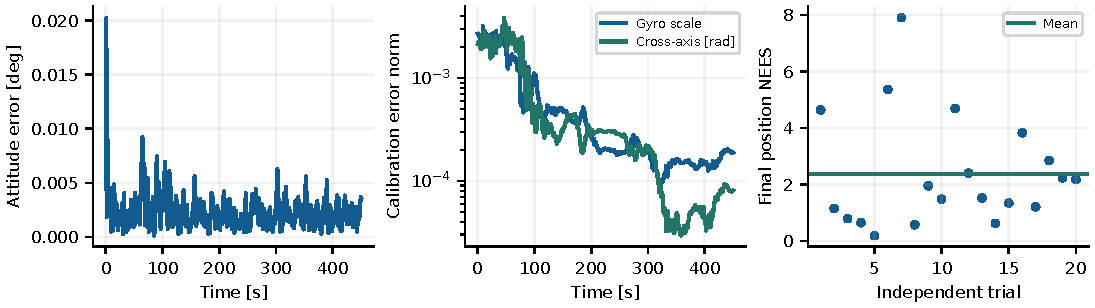
\includegraphics[width=\linewidth]{images/results_navigation_validation.pdf}
\captionof{figure}{Independent navigation fixtures. Left and middle: bounded analytic three-axis attitude with nonzero gyro bias, scale and cross-axis errors; calibration errors converge under the specified excitation and aiding. Right: one final position NEES per independent realization, with their mean. This is separate from the nominal mission and is not a wind/landing robustness ensemble.}
\label{fig:independent-navigation}
\end{minipage}\par\medskip

\subsection{Numerical sensitivity and demonstrated scope}
A saved variant, \path{results/two-stage-final-check}, uses $0.05\,\mathrm{s}$ steps and 20 Hz IMU with matching compared core-physics input hashes. It also lands, at $465.1900\,\mathrm{s}$, with target error $6.171\,\mathrm{m}$ and tilt $1.806^\circ$, versus R1's $3.306\,\mathrm{m}$ and $0.535^\circ$. The plan differs in IMU rate and the integration step is also changed. This is a joint step/clock diagnostic, not an isolated RK4 convergence-order study; contact metrics remain numerically sensitive even when both cases pass.

An isolated constant-spin rigid-body fixture tests RK4 without sensor, guidance or event clocks. Against the exact quaternion at $10\,\mathrm{s}$, steps $0.4$, $0.2$ and $0.1\,\mathrm{s}$ give attitude errors $5.1093\times10^{-7}$, $3.1983\times10^{-8}$ and $1.9997\times10^{-9}\,\mathrm{rad}$. Step-halving orders are 3.9977 and 3.9994, within the selected $[3.8,4.2]$ criterion. This verifies fourth-order behavior in the smooth rotation fixture; it does not establish mission-wide convergence through discrete events.

A separate static allocation check quantifies the dry-CG uncertainty of Section~\ref{sec:vehicle}. With an assumed $10\,\mathrm{t}$ of propellant remaining, the booster mass is $32.2\,\mathrm{t}$ and nominal CG station $16.211\,\mathrm{m}$. Moving the unallocated $6450\,\mathrm{kg}$ centroid over the declared $4.0$--$40.8\,\mathrm{m}$ interval shifts the combined CG by up to $\pm3.686\,\mathrm{m}$. For an explicitly assumed $1\,\mathrm{kN}$ transverse force at a fixed structural station, this changes its CG moment by up to $\pm3.686\,\mathrm{kN\,m}$. These are conditional allocation effects, not flight-error confidence bounds.
            % Ch 9 - to be written
%\section{Engineering Assessment and Implications for Future GNC}
\label{sec:assessment}

\subsection{What the demonstrated results support}
The conservation audit and ascent calibration support controlled model/estimator investigations, rather than mission-wide physical validation. The successful contact in Table~\ref{tab:landing-results} uses physical-state feedback and ideal moments; navigation is evaluated separately. Its assumed initial alignment and zero accepted star fixes further bound the aiding claim. These distinctions define the simulator's role as the Project~2 foundation for later guidance and control \cite[slides 2--4]{project2}.

\subsection{Most dangerous modeling and navigation errors}
For the assignment's final question \cite[slide 8]{project2}, the most dangerous errors are incorrect thrust or measurement directions caused by frame or attitude mistakes, and demands beyond physical actuator authority. This assessment concerns consequences; no failure probabilities are estimated. Table~\ref{tab:gnc-risks} connects the risk pathways to the evidence.

\par\medskip\noindent\begin{minipage}{\linewidth}
\centering\small
\begin{tabularx}{\linewidth}{@{}p{0.20\linewidth}p{0.37\linewidth}X@{}}
\toprule
Error pathway & Evidence or present scope & Consequence for future GNC \\
\midrule
Attitude, rate or frame mismatch & Body-to-$E$ convention is shared; inertial-gyro Earth rate is approximated. The calibrated rate RMS exceeds the raw rate RMS in R1. & Thrust, specific force and lever-arm corrections can point in the wrong direction; attitude accuracy alone does not certify rate feedback. \\
Unavailable control authority & Section~\ref{sec:mission-exec} uses an unlimited ascent couple and bounded ideal return moments, without nozzle/servo dynamics. & Guidance may request impossible turns; control gains can conceal lag, saturation and loss of authority. \\
CG, inertia, flow or thrust error & The conditional $10\,\mathrm{t}$-propellant allocation check shifts CG by up to $3.686\,\mathrm{m}$; the engine and internal geometry are mixed-source estimates. & Force arms, angular acceleration, stopping distance and usable fuel change together, potentially invalidating ignition and reserve predictions. \\
Misleading uncertainty or rejected aiding & All 381 valid star fixes are rejected; reported position envelopes frequently understate error. & Altitude or vertical-speed bias can mis-time braking; overconfidence or failed aiding acquisition can hide that risk despite small nominal RMS error. \\
Aero, wind, event or timing mismatch & Return coefficients are assumed, R1 is calm, and the joint step/IMU-rate variant changes contact metrics. & Lateral miss, loads and burn timing can exceed nominal margins even when the saved nominal run passes. \\
\bottomrule
\end{tabularx}
\captionof{table}{Consequence-based GNC risk assessment grounded in Sections~\ref{sec:vehicle}--\ref{sec:results}. Proposed consequences are engineering reasoning; no probabilities or unperformed robustness results are assigned.}
\label{tab:gnc-risks}
\end{minipage}\par\medskip

\subsection{Recommended progression to guidance and control design}
The first recommendation is to validate the estimator before connecting it to control. Tolerance-based finite-difference checks should cover the propagation, sensor and injection/reset Jacobians. Star-tracker frame, epoch, residual and gate behavior should be isolated in controlled fixtures. Correlated GNSS error and unestimated accelerometer scale error should then be reconciled with the filter uncertainty model. Full covariance, innovation and aiding-acceptance histories are needed for multi-seed consistency studies; a low mean error is insufficient.

The second recommendation is to replace ideal moment authority with a physical allocation and actuator model before tuning vehicle control. The model should resolve available engine/gimbal and fin authority, response rate and saturation, and retain the independently calculated CG/inertia rather than treating inversion of inertia as evidence of stability. The $0.902\,\mathrm{m\,s^{-1}}$ nominal horizontal contact speed against the $1\,\mathrm{m\,s^{-1}}$ project limit leaves little demonstrated margin for these omitted effects.

Finally, a step-size study should hold sensor/guidance clocks fixed, while sensor-rate studies should hold physical integration settings fixed. Mass allocation, thrust, return coefficients and nonzero wind should be varied before multi-seed navigation-fed trials. Independent flight evidence should be reserved for validation after calibration. These recommended studies are not completed evidence; Appendix~\ref{sec:appendix} identifies their controlled inputs.
         % Ch 10 - to be written
%\section{Conclusions}
\label{sec:conclusions}

Project~2 establishes a physics-driven Falcon~9/Dragon simulator and a sensor-driven navigation system for the selected CRS-10 scenario. Forces and moments generate motion through six-degree-of-freedom equations; changing propellant inventories determine mass, CG and inertia; configuration events preserve inherited child states. The simulator therefore generates the trajectory from its models and commands rather than replaying a prescribed flight record. The shared conventions, module interfaces and reproducible execution provide the computational foundation required for subsequent guidance and control development \cite[slides 2--4]{project2}.

The demonstrated mission connects ascent, shutdown, separation, booster return and contact, while independently continuing stage~2 and Dragon to $600\,\mathrm{s}$. The model/navigation and environment suites total 171 passing assertion-based tests. The separation audit satisfies the selected conservation criteria, and the nominal booster meets all declared contact limits. The isolated quaternion fixture exhibits fourth-order RK4 convergence. These checks verify the implemented scenario and interfaces, rather than certify real Falcon~9 separation or landing performance.

The public ascent comparison quantifies the available external evidence: altitude RMSE is $1.577\,\mathrm{km}$ and speed RMSE is $18.46\,\mathrm{m\,s^{-1}}$ over the retained interval. Because this record also informs the ascent calibration, it is not an independent validation set. The return sequence, upper-stage commands and internal mass distribution remain evidence-qualified research models rather than reconstructed CRS-10 flight software or measured mission internals.

Navigation propagates noisy gyro measurements and its own attitude, aided by GNSS, valid LiDAR and 381 accepted star fixes. The nominal IMU-station errors are $\PositionRMS\,\mathrm{m}$ position RMS, $\VelocityRMS\,\mathrm{m\,s^{-1}}$ velocity RMS and $\AttitudeRMS^\circ$ attitude RMS. Final attitude error is $\AttitudeFinal^\circ$, compared with $\GyroOnlyFinal^\circ$ for the paired unaided quaternion. Independent nonzero-error fixtures demonstrate accelerometer/gyro calibration within stated tolerances, and 20 independent realizations pass the position-marginal ANEES test. Nominal calibrated instantaneous rate RMS remains slightly above raw RMS; calibration benefit is demonstrated in the separate nonzero-error fixture. Accuracy, consistency, aiding and parameter observability therefore remain distinct claims.

The principal engineering outcome is a traceable environment in which those distinctions can be investigated. Mixed-source mass properties, assumed return aerodynamics, calm nominal wind, ideal moments and truth-state command feedback limit extrapolation to integrated GNC. Physical actuator modeling, broader uncertainty/outage trials and independent flight validation are justified next steps before closing the navigation-to-control loop. Within this boundary, the project delivers the vehicle, environment, measurement, estimation and numerical interfaces, quantified tests and an auditable assumption/source register. The archived raw evidence and executable figure/validation scripts make the reported results reproducible from a fresh checkout.
        % Ch 11 - to be written
% further chapters are inserted here in document order
% Bibliography. Only verifiable sources; entries follow the evidence
% records in doc/parameter_evidence.md and doc/crs10_mission.md.
\begin{thebibliography}{99}
\small
\setlength{\itemsep}{0pt}
\setlength{\parsep}{0pt}

\bibitem{nasacrs10press}
National Aeronautics and Space Administration:
SpaceX CRS-10 Press Kit, February 2017.
\url{https://www.nasa.gov/wp-content/uploads/2018/07/crs10presskitfinal.pdf}

\bibitem{nasacrs10overview}
National Aeronautics and Space Administration:
SpaceX CRS-10 Mission Overview, 2017.
\url{https://www.nasa.gov/wp-content/uploads/2018/07/spacex_crs-10_mission_overview_0.pdf}

\bibitem{kyledatasheet}
Kyle, E.:
Space Launch Report -- Falcon 9 v1.2 Data Sheet (NASA SMA-hosted copy).
\url{https://sma.nasa.gov/LaunchVehicle/assets/spacex-falcon-9-v1.2-data-sheet.pdf}

\bibitem{crs1presskit}
SpaceX / National Aeronautics and Space Administration:
SpaceX CRS-1 Press Kit, 2012.
\url{https://www.nasa.gov/wp-content/uploads/2015/06/694074main_spacexcrs-1presskit.pdf}

\bibitem{spacexguide2025}
SpaceX:
Falcon User Guide, May 2025.
\url{https://www.spacex.com/assets/media/falcon-users-guide-2025-05-09.pdf}

\bibitem{spacex2015}
SpaceX:
Falcon 9 Payload User's Guide, Rev.~2, October 2015.
\url{https://device.report/m/08e51aa8dc266d701619331c9fdf0c23ce8456f61c08bd14084c00cc7c4d36ae.pdf}

\bibitem{pezent2024}
Pezent, J.:
On the Implementation and Applications of a High Performance Trajectory
Optimization Toolkit.
Ph.D.\ dissertation, The University of Alabama, Tuscaloosa, 2024.
\url{https://ir-api.ua.edu/api/core/bitstreams/cafcf02b-b6e7-47d8-a41b-24b1ba12a154/content}

\bibitem{bykerk2023}
Bykerk, T.:
A standard model for the investigation of aerodynamic and aerothermal loads
on a re-usable launch vehicle.
European Conference for Aeronautics and Space Sciences (EUCASS), 2023.
\url{https://www.eucass.eu/doi/EUCASS2023-018.pdf}

\bibitem{romerocalco2023}
Romero-Calvo et al.:
Novel propellant settling strategies for liquid rocket engine restart in
microgravity, 2023.
\url{https://hanspeterschaub.info/PapersPrivate/RomeroCalvo2023.pdf}

\bibitem{ussa1976}
U.S.\ Committee on Extension to the Standard Atmosphere:
U.S.\ Standard Atmosphere, 1976.
U.S.\ Government Printing Office, Washington, D.C., 1976.
\url{https://ntrs.nasa.gov/citations/19770009539}

\bibitem{project2}
Hyeongjun Park, \emph{Project 2: Development of Vehicle Simulator with Navigation Blocks}, Guidance, Navigation, and Control System for Reusable Launch Vehicles, Seoul National University, course slides 2--8.

\bibitem{nasacrs10photo}
NASA/Glenn Benson, \emph{Falcon 9 Rocket Ready for SpaceX CRS-10}, 18 February 2017.
\url{https://www.nasa.gov/image-article/falcon-9-rocket-ready-spacex-crs-10-2/}

\bibitem{crs10webcast}
SpaceX, \emph{CRS-10 Technical Webcast}, 19 February 2017.
\url{https://www.youtube.com/watch?v=rUDLxFUMC9c}

\bibitem{crs10telemetry}
shahar603, \emph{Telemetry-Data: SpaceX CRS-10}, author-published webcast digitization, revision \texttt{b245d3b81aa36b7941ec10f3f4b508999d106a6d}.
\url{https://github.com/shahar603/Telemetry-Data/tree/b245d3b81aa36b7941ec10f3f4b508999d106a6d/SpaceX%20CRS-10}

\bibitem{ecker2017}
T. Ecker, S. Karl, E. Dumont, S. Stappert, and D. Krause, ``A Numerical Study on the Thermal Loads During a Supersonic Rocket Retro-Propulsion Maneuver,'' AIAA 2017-4878, Table 1.
\url{https://doi.org/10.2514/6.2017-4878}

\bibitem{miquel2020}
V. Miquel, \emph{Propellant Feeding System of a Liquid Rocket With Multiple Engines}, KTH Royal Institute of Technology, 2020, Table 5, PDF p.~24.
\url{https://www.diva-portal.org/smash/get/diva2:1440090/FULLTEXT01.pdf}

\bibitem{faa2018}
FAA Office of Commercial Space Transportation, \emph{The Annual Compendium of Commercial Space Transportation: 2018}, Falcon 9 FT fact sheet. Retained legacy dimensional source chain; stage-boundary applicability to CRS-10 is conditional.
\url{https://www.faa.gov/about/office_org/headquarters_offices/ast/media/2018_AST_Compendium.pdf}

\bibitem{rocketpyeom}
RocketPy developers, \emph{Equations of Motion v1}, technical documentation, accessed 10 November 2026.
\url{https://docs.rocketpy.org/en/latest/technical/equations_of_motion_v1.html}

\end{thebibliography}



\end{document}
